\documentclass[dvipdfmx,a4paper]{ujarticle}

\usepackage{mymacro}
\usepackage{graphicx}
\usepackage[dvipdfmx]{color}
\usepackage{xcolor}
\usepackage{here} % \begin{figure}[H]
\usepackage{ascmac} % \boxnote ほか
\usepackage{listings, jlisting}
%\usepackage{multicol}
%% -- \url link
\usepackage[linkcolor=black]{hyperref}
\usepackage[hyperrefcolorlinks,os=win]{menukeys}
\usepackage{pxjahyper}
%% --
\lstset{language=c,
  breaklines = true,
  linewidth=\textwidth,
  xleftmargin=20pt,
  xrightmargin=20pt,
  basicstyle={\footnotesize\ttfamily},
  identifierstyle={\footnotesize\ttfamily},
  commentstyle={\footnotesize\ttfamily},
  keywordstyle={\footnotesize\ttfamily},
  ndkeywordstyle={\footnotesize\ttfamily},
  stringstyle={\footnotesize\ttfamily},
  classoffset=1,
  frame=tRBl,
  framesep=5pt,
  showstringspaces=false,
  numbers=left,
  stepnumber=1,
  tabsize=4
}
%%
%%%%%%%%%%%%%%%%%%%%%%%%%%%%%%%%%%%%%%%%%%%%%
% 図番号,表番号を章番号付きで
%%%%%%%%%%%%%%%%%%%%%%%%%%%%%%%%%%%%%%%%%%%%%
\renewcommand{\theequation}{\arabic{section}.\arabic{equation}}
\renewcommand{\thefigure}{\arabic{section}.\arabic{figure}}
\renewcommand{\thetable}{\arabic{section}.\arabic{table}}
\makeatletter
\@addtoreset{equation}{section}
\@addtoreset{figure}{section}
\@addtoreset{table}{section}
% listings用の設定
\AtBeginDocument{
  \renewcommand*{\thelstlisting}{\arabic{section}.\arabic{lstlisting}}%
  \@addtoreset{lstlisting}{section}
}
\makeatother

\begin{document}

\thispagestyle{empty}
%!TEX root = ./NCVC.tex

\vspace*{4zh}
\begin{figure}[H]
\centering

\includegraphics[scale=1.2]{logo.png}
\end{figure}

\vspace*{3zh}
\begin{center}
    \rule{6cm}{0.2zw}\\[-0.5zh]
    \rule{5cm}{0.1zw}\\[-0.5zh]
    \rule{4cm}{0.05zw}\\[1zh]
    {\Large \textbf{NCVC解説書}}\\
    \rule{4cm}{0.05zw}\\[-0.5zh]
    \rule{5cm}{0.1zw}\\[-0.5zh]
    \rule{6cm}{0.2zw}

    \vspace*{8cm}
    NCVC Ver0.14.42 用\\
    2005 年 10 月 初版
\end{center}

\newpage

\setcounter{page}{0}
\thispagestyle{empty}
{\small \tableofcontents}
\newpage

%!TEX root = ../NCVC.tex

\mysection{基本編}

\subsection{CADでの作図}

\begin{minipage}[t]{0.4\textwidth}
 まずは基本的な加工を行うための基本的な作図方法を解説します.
図\ref{fig:sample1.jww} のような図形を書きましょう.
切削対象(ワーク)を示す矩形と,その矩形左下に円を1つ.
「NCVC」という文字は,線をつなぎ合わせたデータです.
\end{minipage}
\begin{minipage}[t]{0.6\textwidth}
\vspace*{-2zh}
\begin{figure}[H]
\centering
\includegraphics[scale=0.8]{No1/fig/sample1.pdf}
\caption{サンプル図形}
\label{fig:sample1.jww}
\end{figure}
\end{minipage}

\vspace*{2zh}
 NCVCはCADでの作図情報を全て読み込むのではなく,
特定のレイヤ情報を元に作図データを読み込みます.
CADでの作図において必要とされる補助線や寸法線等が加工データには必要なく,
これらを選別するための仕様です.

 その選別方法は『必要なレイヤに名前を付ける』こと.
図\ref{fig:sampleLayer.png} は図\ref{fig:sample1.jww} のレイヤ情報ですが,
0番レイヤに「ORIGIN」という名前,
1番レイヤに「CAM\_LINE」という名前を付けています.
それぞれ機械原点と切削軌跡を示し,この2つのレイヤは必須です
\footnote{実は機械原点レイヤは必須ではありません.詳細は【穴加工】の節で解説しています.}.
機械原点レイヤには工作機械のXY原点を示す円を1つだけ作図.
大きさは任意ですが,円の中心がXYの原点となります.
切削軌跡 CAM\_LINE レイヤには刃物のパス,
すなわち削りたい図形を書きます.
他,ワーク矩形を示す補助線等は別のレイヤに書きます.
レイヤに名前を付ける方法は,それぞれのCAD操作に準拠して下さい.
なお,全てのデータにおいて線種,線色は関係ありません.

\vspace*{1zh}
\begin{figure}[H]
\centering
\includegraphics{No1/fig/sampleLayer.png}
\caption{レイヤ一覧}
\label{fig:sampleLayer.png}
\end{figure}

 作図が終わればCADデータをDXF形式で保存します
\footnote{
    Jw\_cadの場合,DXF形式で保存する必要はありません.NCVCはJWW形式を直接読み込むことが可能です.
    詳細は【パワーユーザ編】の【アドイン作成のすすめ】を参照して下さい.
}.
NCVCにCADデータを読み込ませるためDXF形式で保存する必要がありますが,
多くの場合,DXF形式で保存するとそのCAD独自のデータが失われるため,
使用しているCAD独自の形式でも保存しておきましょう.

\subsection{CADデータの読み込み}

\begin{minipage}[t]{0.5\textwidth}
 NCVCでDXF形式のCADデータを読み込みます.
が,その前に確認.
NCVCの \menu{オプション>DXF関連の設定} をクリックし,
NCVCが読み込むレイヤ名を設定して下さい.
デフォルトで先ほど設定した値になっていると思います.
基本編では[従来互換]のみ解説しますので,図\ref{fig:NCVCsetup.png} の通り設定して下さい.
この値は任意です.CAD側の設定と合わせて下さい.
無事読み込めると原点を示す十字(大きさは原点円の直径)と切削対象のパスが表示されます.
原点レイヤと切削レイヤ以外に作図した情報,
例えば,図\ref{fig:sampleLayer.png} の4番レイヤに書いたワークを表す矩形は読み込まれません(図\ref{fig:NCVCread.png}).
CADでの線種・線色は無視され,NCVCの設定に基づき表示されます.
詳細はリファレンスの表示属性を参照してください.
\end{minipage}
\begin{minipage}[t]{0.5\textwidth}
\vspace*{-2zh}
\begin{figure}[H]
\centering
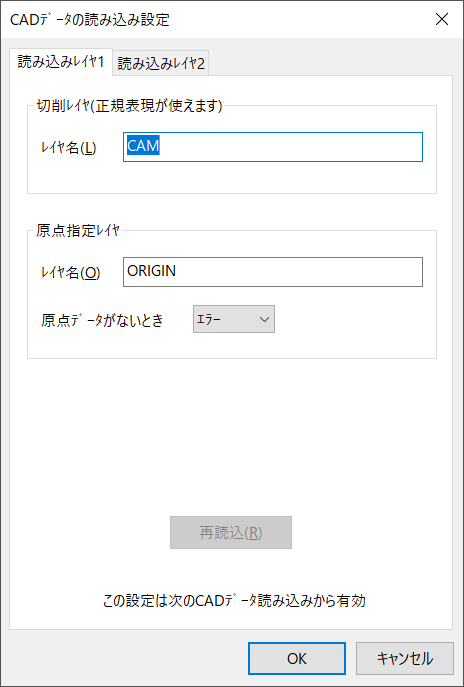
\includegraphics[scale=0.8]{No1/fig/NCVCsetup.png}
\caption{読み込みレイヤ設定}
\label{fig:NCVCsetup.png}
\end{figure}
\end{minipage}

\begin{figure}[H]
\centering
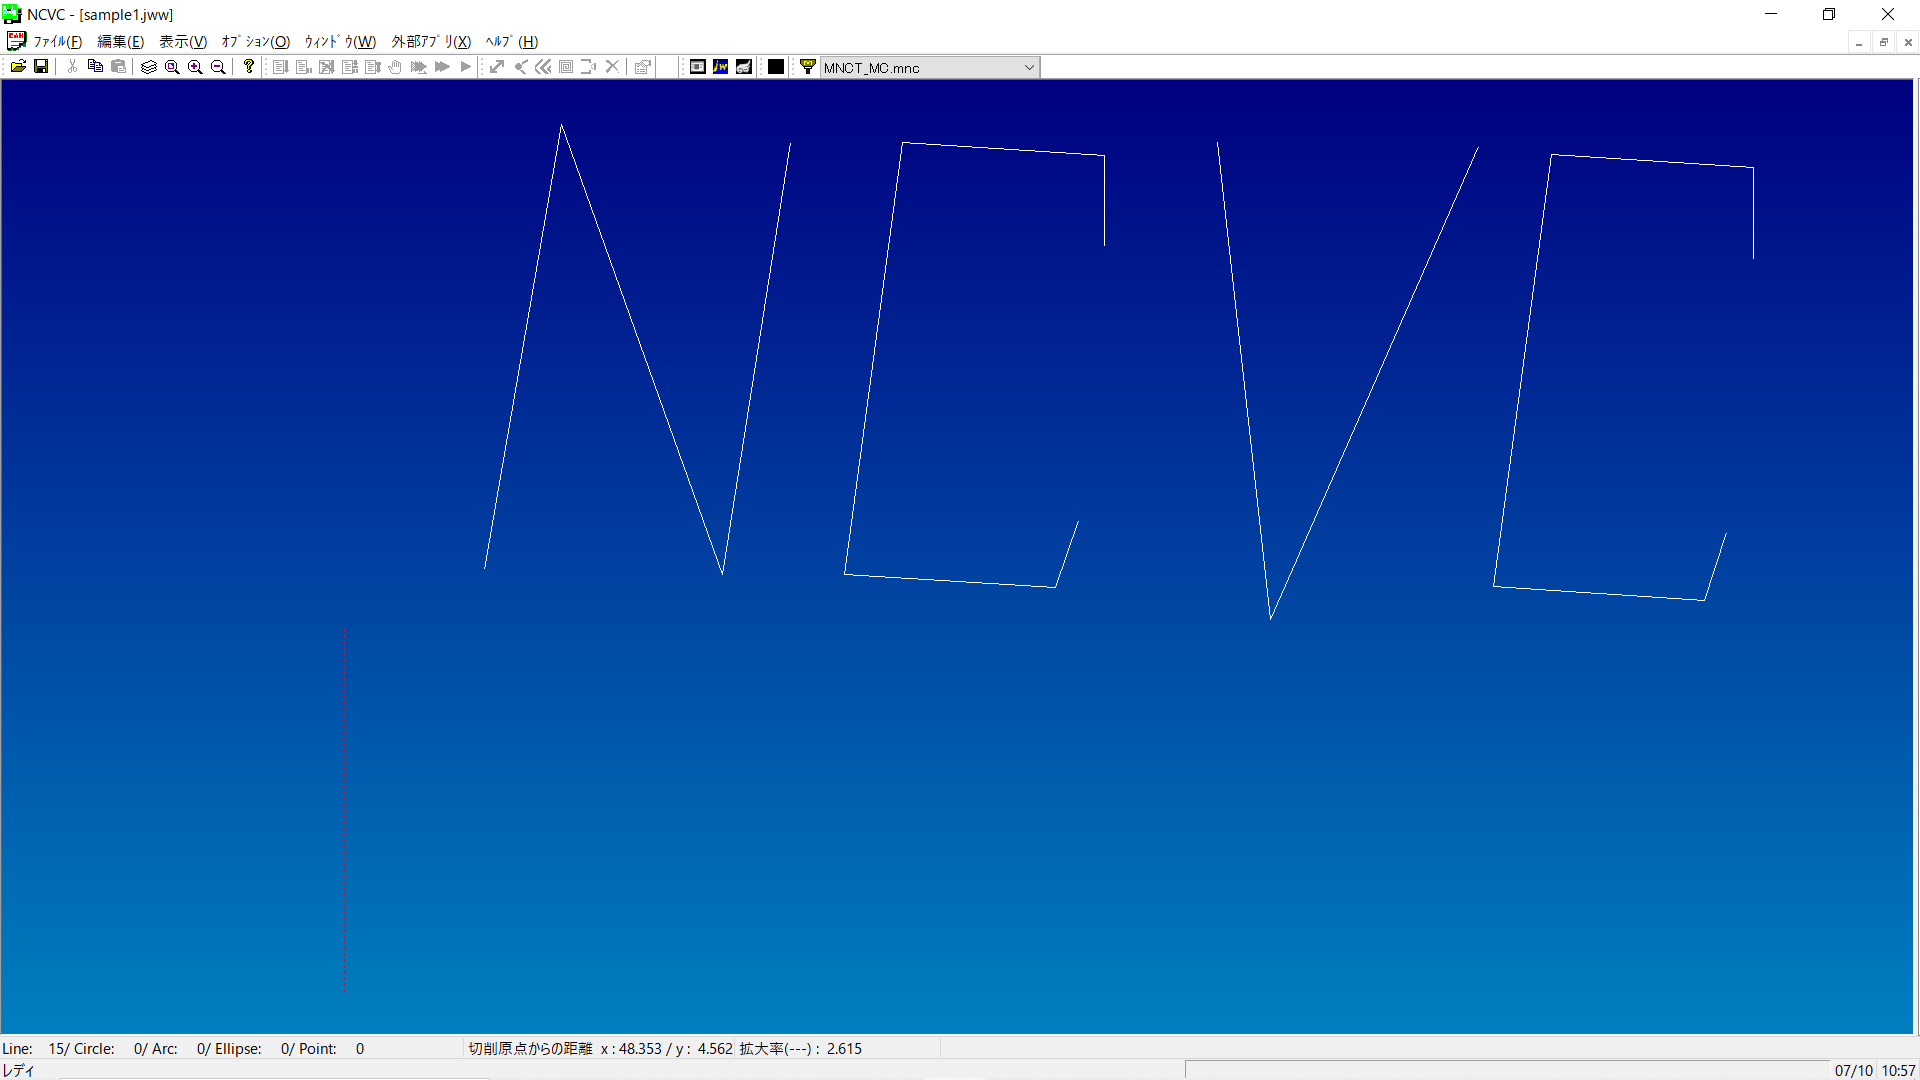
\includegraphics[scale=0.4]{No1/fig/NCVCread.png}
\caption{CADデータの読み込み}
\label{fig:NCVCread.png}
\end{figure}

\subsection{加工条件の設定}

 いよいよCADデータからGコードを生成するわけですが,ご覧の通り読み込んだCADデータは2次元です.
工作機械のZ軸方向の移動はどうやって制御するのでしょうか?
答えは[加工条件]の中にあります.
\menu{オプション>切削パラメータの設定} をクリックし,条件ファイル(nciファイル)を選択します.
標準で用意されている[Init.nci]の設定を変更しましょう.

 条件ファイルを選択すると図\ref{fig:init.nci.png} のダイアログが表示されます.
ここで重要なのが切削原点(G92)のZ値とR点,切り込みパラメータの3つです.

 図\ref{fig:XZ-crop.pdf} は工作機械を正面から見た図,上下にZ軸,左右にX軸です.
ワークをセットしたあと,ワーク平面を基準にZセンサー等でZ軸の位置決めを行います.
これを切削原点(G92)のZ値とします.
Zセンサーの厚みが100mmなら100と入力です.
センサーでの調整後,好みの位置に移動させてもかまいません.
無論そのときは移動した座標値を入力して下さい.

 次に切り込みですが,イメージ通り.ワークに何ミリ切り込むかという設定です.
最後にR点ですが,これは次の切削領域,この例で言うと``\,N\,''を削って``\,C\,''に移動するときのZ値を指定します.
Z軸の初期位置(原点)で移動してもかまわないのですが,初期位置は高く設定する傾向があるため,効率よく移動できる下限値と考えて下さい.
この設定ではワーク平面上空1mmの所で刃物が次の切削領域へ高速移動します.

 ワーク平面を基準に値を選びましたが,Zセンサー調整後の位置を基準,
すなわち,ワーク上空10mmの位置をZ軸の原点(G92Zをゼロ)としたとき,この例ではR点が-9mm,切り込みは-12mmとなります.
意味は同じですから各自の好みや考えやすい方で指示して下さい.

 他,主軸回転数や送り速度など,ワーク材質に合わせて設定します.

\begin{minipage}{0.5\textwidth}
\begin{figure}[H]
\centering
\includegraphics[scale=0.7]{No1/fig/init.nci.png}
\caption{加工条件の設定}
\label{fig:init.nci.png}
\end{figure}
\end{minipage}
\begin{minipage}{0.5\textwidth}
\begin{figure}[H]
\centering
\includegraphics[scale=0.8]{No1/fig/XZ-crop.pdf}
\caption{Z軸における各パラメータの関係}
\label{fig:XZ-crop.pdf}
\end{figure}
\end{minipage}

\subsection{Gコードの生成}

\begin{minipage}[t]{0.5\textwidth}
 加工条件の設定ができればあとはNCVCの仕事.
\menu{ファイル>NCデータへの変換>単一条件(従来互換)} をクリック.
出力ファイル名(自動設定)と条件ファイルを指定(図\ref{fig:make.png})し,OKをクリックすれば
\end{minipage}
\begin{minipage}[t]{0.5\textwidth}
\vspace*{-2zh}
\begin{figure}[H]
\centering
\includegraphics[scale=0.7]{No1/fig/make.png}
\caption{Gコードの出力と条件ファイルの指示}
\label{fig:make.png}
\end{figure}
\end{minipage}

\vspace*{2zh}
 おめでとうございます!見事Gコードが生成できました.
図\ref{fig:make.png} で[NC生成後に開く]にチェックが入っていると,即座に結果を確認することが出来ます.
図\ref{fig:sim.png} にGコードのシミュレーション結果を示します.

\begin{figure}[H]
\centering
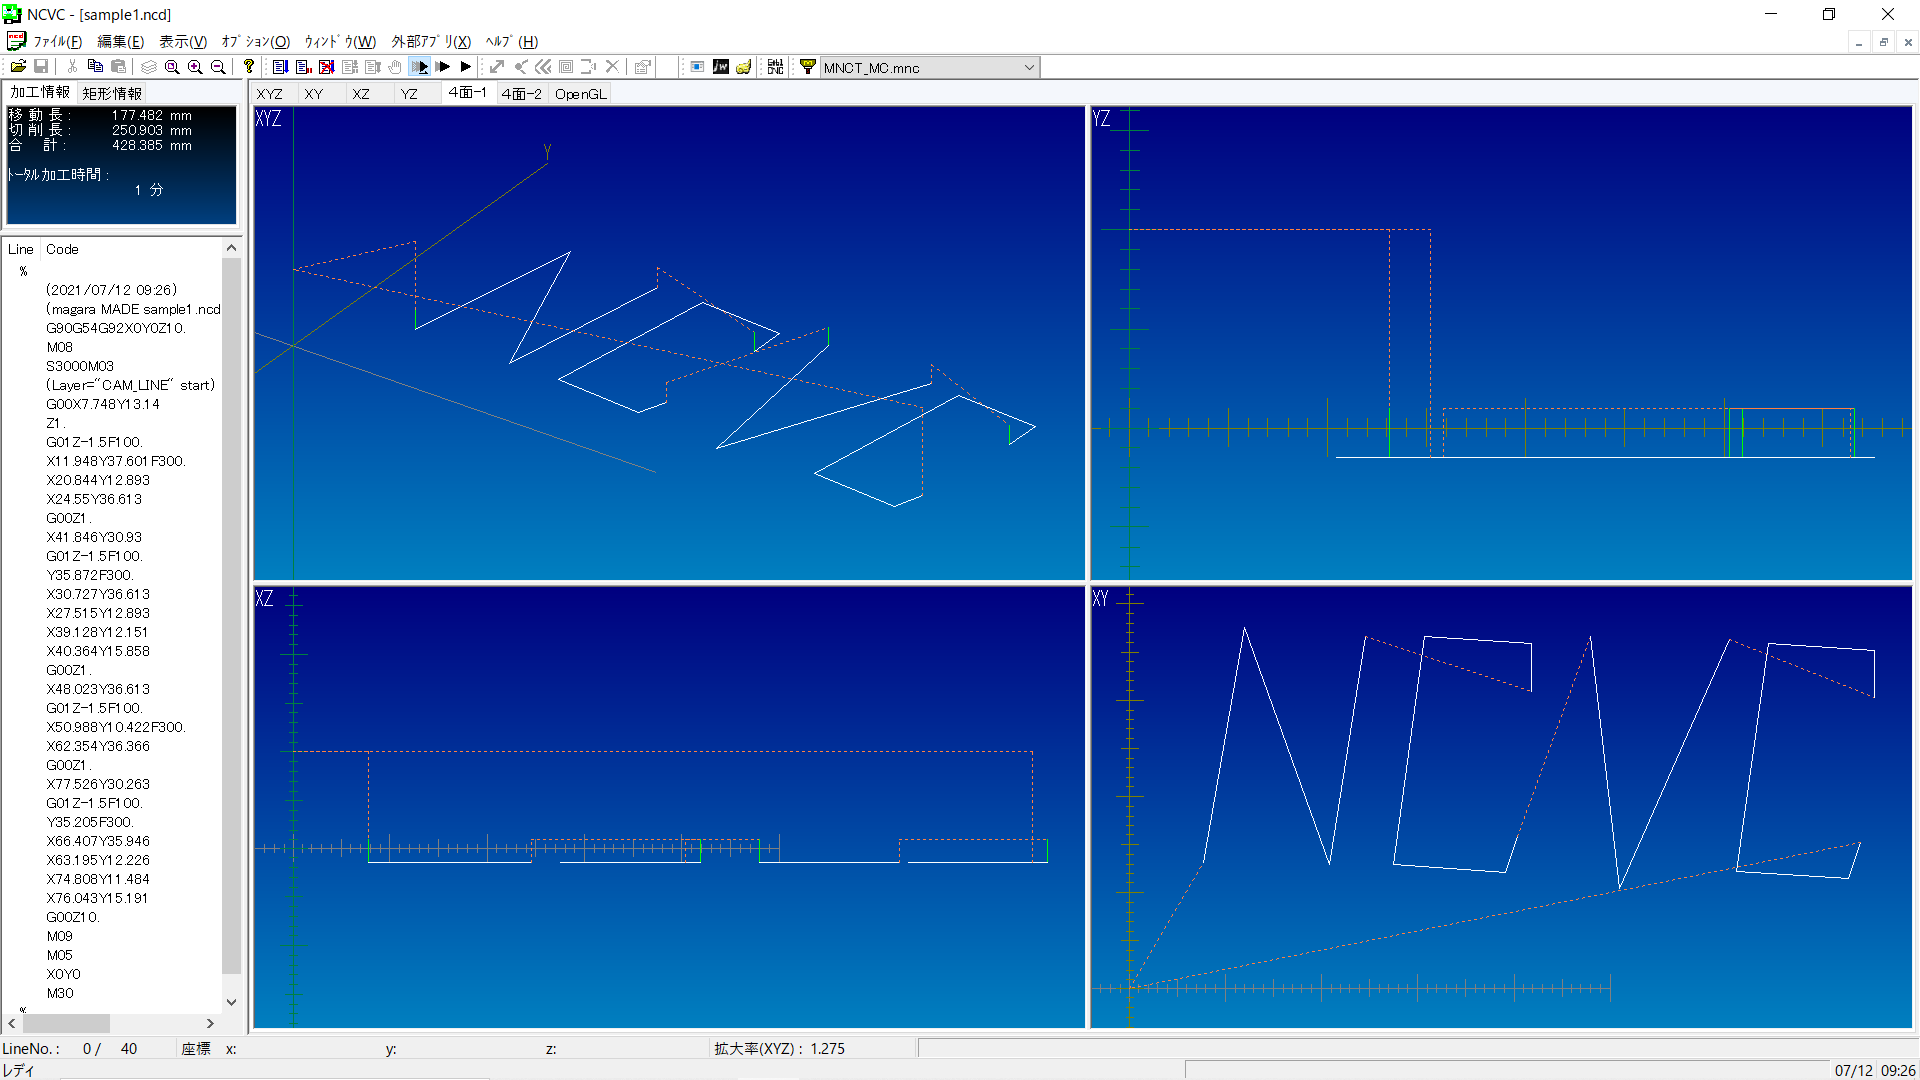
\includegraphics[scale=0.4]{No1/fig/sim.png}
\caption{Gコードシミュレーション画面}
\label{fig:sim.png}
\end{figure}

\vspace*{2zh}
\begin{itembox}[l]{ここまでの【まとめ】}
(1) CADでの操作
\begin{itemize}
\item 工作機械のXY原点を示す円を原点レイヤに作図
\item 刃物の軌跡を切削レイヤに作図
\item 原点レイヤと切削レイヤに名前を付ける
\item 線種・線色は無視され,NCVCの表示属性により表示される
\end{itemize}
(2) NCVCでの操作
\begin{itemize}
\item CADデータを読み込むために,読み込みレイヤの設定を行う
\item Z軸の原点や切り込み量は加工条件で設定する
\end{itemize}
\end{itembox}

\subsection{加工条件の設定2}

 ところで図\ref{fig:sim.png} の左,Gコードのリストに注目すると,
G54ワーク座標系選択やMコードなど,CADでの作図データ以外のコードが生成されています.
これらの設定は加工条件(図\ref{fig:init.nci.png})のヘッダー・フッターの両カスタムファイルによるものです.
以下のリスト,標準で用意されているカスタムファイルで,左がヘッダー,右がフッターです.
それぞれ生成開始時と終了時に参照され,生成するGコードに併合されます.
使用できる置換キーワードなど詳細は第5章の【リファレンス】で解説します.

\begin{minipage}[t]{0.75\textwidth}
\begin{lstlisting}[caption=Header.txt,numbers=none,label=lst:header.txt]
%
({MakeDate} {MakeTime})
({MakeUser} MADE {MakeNCD} FROM {MakeDXF} AND {MakeCondition})
{G90orG91}G54{G92_Initial}
M8
{Spindle}M3
\end{lstlisting}
\end{minipage}
\begin{minipage}[t]{0.25\textwidth}
\begin{lstlisting}[caption=Footer.txt,numbers=none,label=lst:footer.txt]
M9
M5
{G0XY_Initial}
M30
%
\end{lstlisting}
\end{minipage}

 テキストファイルなのでメモ帳などで編集できます.
例えばワイヤー加工機のワイヤー設定,レーザー加工機の出力設定など,ヘッダー・フッターファイルで指定しなければならない設定は多々あると思います.
実際の運用では,加工条件ファイルを含め,対象となる工作機械ごとに設定ファイルを用意する方が良いでしょう.
本解説書では標準ヘッダーにチップコンベア起動の``\,M68\,''を挿入しています.
他,そのまま使っても問題無いと思いますが,見づらいようならコメント行(ヘッダーの2~3行目)は削除してもかまいません.

 生成時に図\ref{fig:error.png} のようなエラーメッセージが出る場合があります.
特に標準のインストールパス以外にインストールされた場合,両カスタムファイルが探せませんので,加工条件にて正しいパスを設定して下さい.

\begin{figure}[H]
\centering
\includegraphics{No1/fig/error.png}
\caption{カスタムファイルのエラーメッセージ}
\label{fig:error.png}
\end{figure}

\newpage

%!TEX root = ../NCVC.tex

\mysection{基本編}

\subsection{CADでの作図}
\label{DesignCAD}

\begin{minipage}[t]{0.4\textwidth}
 まずは基本的な加工を行うための基本的な作図方法を解説します.
図\ref{fig:sample1.jww} のような図形を書きましょう.
切削対象(ワーク)を示す矩形と,その矩形左下に円を1つ.
「NCVC」という文字は,線をつなぎ合わせたデータです.
\end{minipage}
\begin{minipage}[t]{0.6\textwidth}
\vspace*{-2zh}
\begin{figure}[H]
\centering
\includegraphics[scale=0.8]{No2/fig/sample1.pdf}
\caption{サンプル図形}
\label{fig:sample1.jww}
\end{figure}
\end{minipage}

\vspace*{2zh}
 NCVCはCADでの作図情報を全て読み込むのではなく,
特定のレイヤ情報を元に作図データを読み込みます.
CADでの作図において必要とされる補助線や寸法線等が加工データには必要なく,
これらを選別するための仕様です.

 その選別方法は『必要なレイヤに名前を付ける』こと.
図\ref{fig:sampleLayer.png} は図\ref{fig:sample1.jww} のレイヤ情報ですが,
0番レイヤに「ORIGIN」という名前,
1番レイヤに「CAM\_LINE」という名前を付けています.
それぞれ機械原点と切削軌跡を示し,この2つのレイヤは必須です
\footnote{実は機械原点レイヤは必須ではありません.詳細は【穴加工】の節で解説しています.}.
機械原点レイヤには工作機械のXY原点を示す円を1つだけ作図.
大きさは任意ですが,円の中心がXYの原点となります.
切削軌跡 CAM\_LINE レイヤには刃物のパス,
すなわち削りたい図形を書きます.
他,ワーク矩形を示す補助線等は別のレイヤに書きます.
レイヤに名前を付ける方法は,それぞれのCAD操作に準拠して下さい.
なお,全てのデータにおいて線種,線色は関係ありません.

\vspace*{1zh}
\begin{figure}[H]
\centering
\includegraphics{No2/fig/sampleLayer.png}
\caption{レイヤ一覧}
\label{fig:sampleLayer.png}
\end{figure}

 作図が終わればCADデータをDXF形式で保存します
\footnote{
    Jw\_cadの場合,DXF形式で保存する必要はありません.NCVCはJWW形式を直接読み込むことが可能です.
    詳細は【パワーユーザ編】の【アドイン作成のすすめ】を参照して下さい.
}.
NCVCにCADデータを読み込ませるためDXF形式で保存する必要がありますが,
多くの場合,DXF形式で保存するとそのCAD独自のデータが失われるため,
使用しているCAD独自の形式でも保存しておきましょう.

\subsection{CADデータの読み込み}
\label{sec:ReadCAD}

\begin{minipage}[t]{0.5\textwidth}
 NCVCでDXF形式のCADデータを読み込みます.
が,その前に確認.
NCVCの \menu{オプション>DXF関連の設定} をクリックし,
NCVCが読み込むレイヤ名を設定して下さい.
デフォルトで先ほど設定した値になっていると思います.
基本編では[従来互換]のみ解説しますので,図\ref{fig:ReadSetup.png} の通り設定して下さい.
この値は任意です.CAD側の設定と合わせて下さい.
無事読み込めると原点を示す十字(大きさは原点円の直径)と切削対象のパスが表示されます.
原点レイヤと切削レイヤ以外に作図した情報,
例えば,図\ref{fig:sampleLayer.png} の4番レイヤに書いたワークを表す矩形は読み込まれません(図\ref{fig:ReadJWW.png}).
CADでの線種・線色は無視され,NCVCの設定に基づき表示されます.
詳細はリファレンスの表示属性を参照してください.
\end{minipage}
\begin{minipage}[t]{0.5\textwidth}
\vspace*{-2zh}
\begin{figure}[H]
\centering
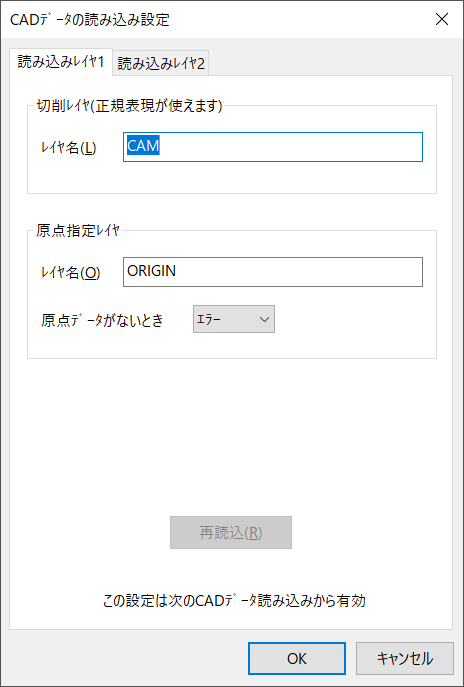
\includegraphics[scale=0.7]{No2/fig/ReadSetup.png}
\caption{読み込みレイヤ設定}
\label{fig:ReadSetup.png}
\end{figure}
\end{minipage}

\begin{figure}[H]
\centering
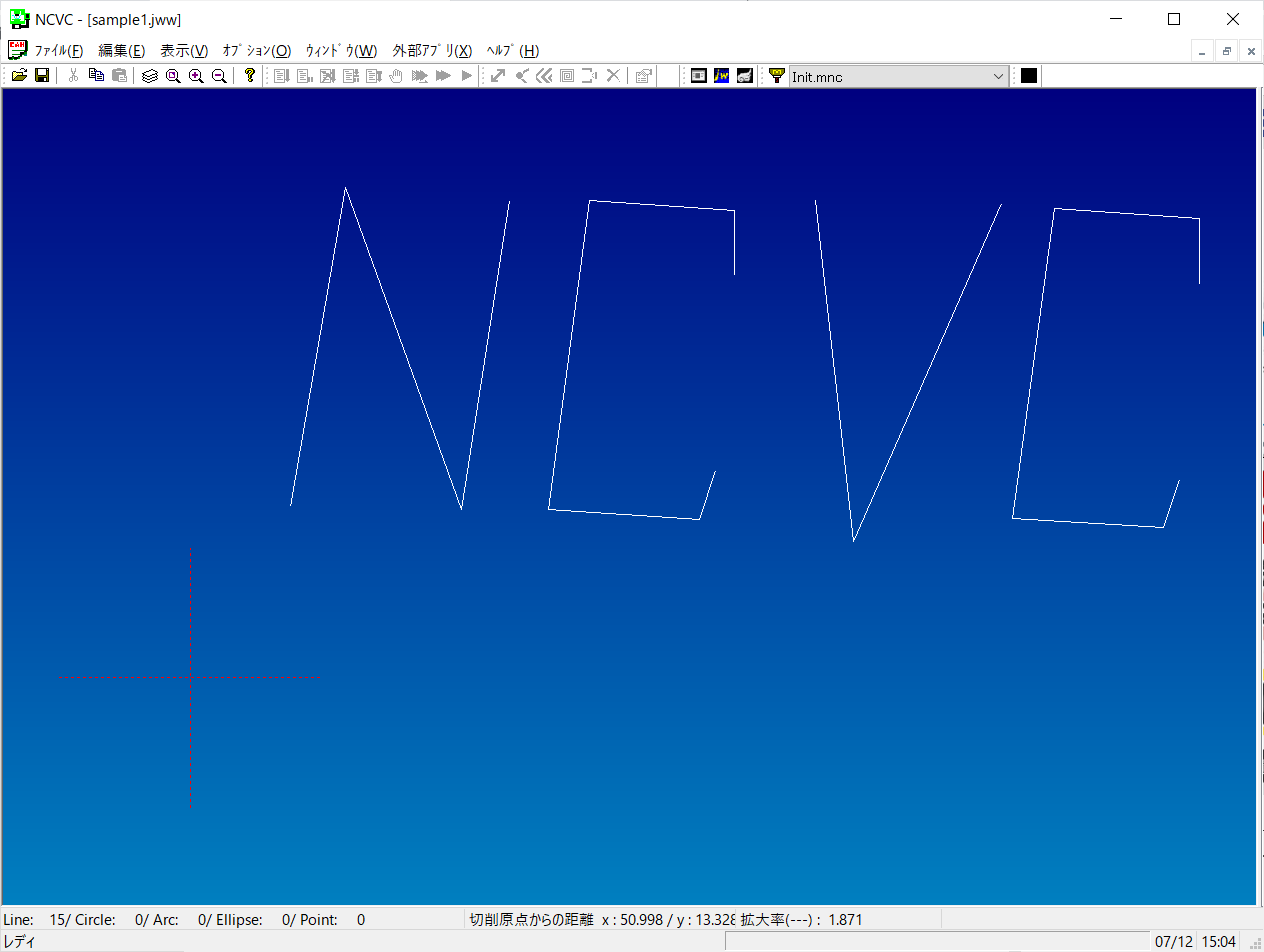
\includegraphics[scale=0.55]{No2/fig/ReadJWW.png}
\caption{CADデータの読み込み}
\label{fig:ReadJWW.png}
\end{figure}

\subsection{加工条件の設定}
\label{sec:init.nci}

 いよいよCADデータからGコードを生成するわけですが,ご覧の通り読み込んだCADデータは2次元です.
工作機械のZ軸方向の移動はどうやって制御するのでしょうか?
答えは[加工条件]の中にあります.
\menu{オプション>切削パラメータの設定} をクリックし,条件ファイル(nciファイル)を選択します.
標準で用意されている[Init.nci]の設定を変更しましょう.

 条件ファイルを選択すると図\ref{fig:init.nci.png} のダイアログが表示されます.
ここで重要なのが切削原点(G92)のZ値とR点,切り込みパラメータの3つです.

 図\ref{fig:XZ-crop.pdf} は工作機械を正面から見た図,上下にZ軸,左右にX軸です.
ワークをセットしたあと,ワーク平面を基準にZセンサー等でZ軸の位置決めを行います.
これを切削原点(G92)のZ値とします.
Zセンサーの厚みが100mmなら100と入力です.
センサーでの調整後,好みの位置に移動させてもかまいません.
無論そのときは移動した座標値を入力して下さい.

 次に切り込みですが,イメージ通り.ワークに何ミリ切り込むかという設定です.
最後にR点ですが,これは次の切削領域,この例で言うと``\,N\,''を削って``\,C\,''に移動するときのZ値を指定します.
Z軸の初期位置(原点)で移動してもかまわないのですが,初期位置は高く設定する傾向があるため,効率よく移動できる下限値と考えて下さい.
この設定ではワーク平面上空1mmの所で刃物が次の切削領域へ高速移動します.

 ワーク平面を基準に値を選びましたが,Zセンサー調整後の位置を基準,
すなわち,ワーク上空10mmの位置をZ軸の原点(G92Zをゼロ)としたとき,この例ではR点が-9mm,切り込みは-12mmとなります.
意味は同じですから各自の好みや考えやすい方で指示して下さい.

 他,主軸回転数や送り速度など,ワーク材質に合わせて設定します.

\begin{minipage}{0.5\textwidth}
\begin{figure}[H]
\centering
\includegraphics[scale=0.7]{No2/fig/init.nci.png}
\caption{加工条件の設定}
\label{fig:init.nci.png}
\end{figure}
\end{minipage}
\begin{minipage}{0.5\textwidth}
\begin{figure}[H]
\centering
\includegraphics[scale=0.8]{No2/fig/XZ-crop.pdf}
\caption{Z軸における各パラメータの関係}
\label{fig:XZ-crop.pdf}
\end{figure}
\end{minipage}

\subsection{Gコードの生成}
\label{sec:MakeGcode}

\begin{minipage}[t]{0.5\textwidth}
 加工条件の設定ができればあとはNCVCの仕事.
\menu{ファイル>NCデータへの変換>単一条件(従来互換)} をクリック.
出力ファイル名(自動設定)と条件ファイルを指定(図\ref{fig:make.png})し,OKをクリックすれば...
\end{minipage}
\begin{minipage}[t]{0.5\textwidth}
\vspace*{-2zh}
\begin{figure}[H]
\centering
\includegraphics[scale=0.7]{No2/fig/make.png}
\caption{Gコードの出力と条件ファイルの指示}
\label{fig:make.png}
\end{figure}
\end{minipage}

\begin{figure}[H]
\centering
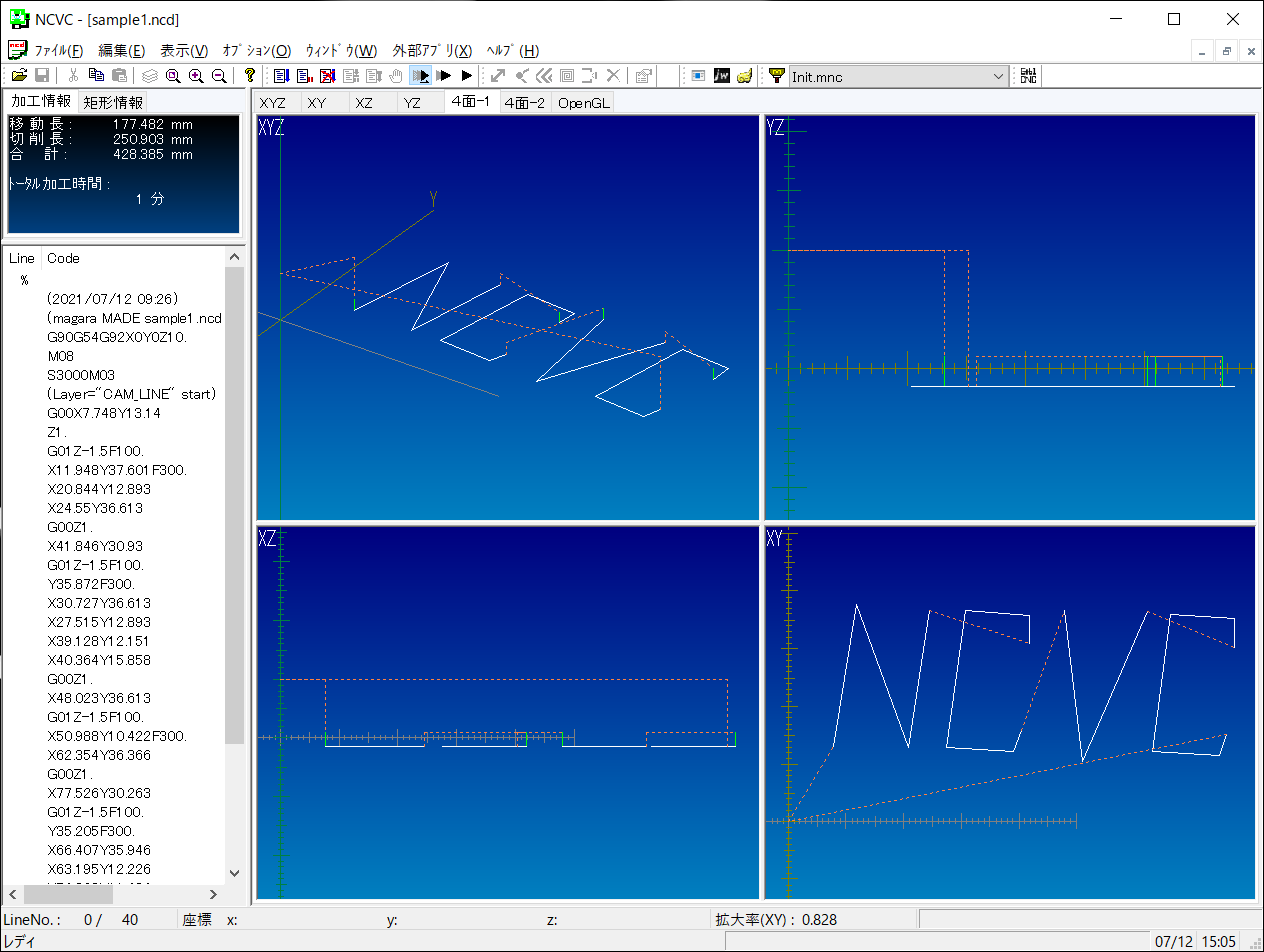
\includegraphics[scale=0.55]{No2/fig/sample01.png}
\caption{Gコードシミュレーション画面}
\label{fig:sample1.png}
\end{figure}

 おめでとうございます!見事Gコードが生成できました.
図\ref{fig:make.png} で[NC生成後に開く]にチェックが入っていると,即座に結果を確認することが出来ます.
図\ref{fig:sample1.png} にGコードのシミュレーション結果を示します.

\vspace*{3zh}
\begin{itembox}[l]{ここまでの【まとめ】}
(1) CADでの操作
\begin{itemize}
\item 工作機械のXY原点を示す円を原点レイヤに作図
\item 刃物の軌跡を切削レイヤに作図
\item 原点レイヤと切削レイヤに名前を付ける
\item 線種・線色は無視され,NCVCの表示属性により表示される
\end{itemize}
(2) NCVCでの操作
\begin{itemize}
\item CADデータを読み込むために,読み込みレイヤの設定を行う
\item Z軸の原点や切り込み量は加工条件で設定する
\end{itemize}
\end{itembox}

\newpage
\subsection{加工条件の設定2}

 ところで図\ref{fig:sample1.png} の左,Gコードのリストに注目すると,
G54ワーク座標系選択やMコードなど,CADでの作図データ以外のコードが生成されています.
これらの設定は加工条件(図\ref{fig:init.nci.png})のヘッダー・フッターの両カスタムファイルによるものです.
以下のリスト,標準で用意されているカスタムファイルで,左がヘッダー,右がフッターです.
それぞれ生成開始時と終了時に参照され,生成するGコードに併合されます.
使用できる置換キーワードなど詳細は第5章の【リファレンス】で解説します.

\begin{minipage}[t]{0.75\textwidth}
\begin{lstlisting}[caption=Header.txt,numbers=none,label=lst:header.txt]
%
({MakeDate} {MakeTime})
({MakeUser} MADE {MakeNCD} FROM {MakeDXF} AND {MakeCondition})
{G90orG91}G54{G92_Initial}
M8
{Spindle}M3
\end{lstlisting}
\end{minipage}
\begin{minipage}[t]{0.25\textwidth}
\begin{lstlisting}[caption=Footer.txt,numbers=none,label=lst:footer.txt]
M9
M5
{G0XY_Initial}
M30
%
\end{lstlisting}
\end{minipage}

\vspace*{2zh}
 テキストファイルなのでメモ帳などで編集できます.
例えばワイヤー加工機のワイヤー設定,レーザー加工機の出力設定など,ヘッダー・フッターファイルで指定しなければならない設定は多々あると思います.
実際の運用では,加工条件ファイルを含め,対象となる工作機械ごとに設定ファイルを用意する方が良いでしょう.
本解説書では標準ヘッダーにチップコンベア起動の``\,M68\,''を挿入しています.
他,そのまま使っても問題無いと思いますが,見づらいようならコメント行(ヘッダーの2~3行目)は削除してもかまいません.

 生成時に図\ref{fig:error.png} のようなエラーメッセージが出る場合があります.
特に標準のインストールパス以外にインストールされた場合,両カスタムファイルが探せませんので,加工条件にて正しいパスを設定して下さい.

\begin{figure}[H]
\centering
\includegraphics{No2/fig/error.png}
\caption{カスタムファイルのエラーメッセージ}
\label{fig:error.png}
\end{figure}

\subsection{Gコードの加工シミュレーション}

\subsubsection{加工時間の表示}

\begin{minipage}[t]{0.5\textwidth}
 図\ref{fig:sample1.png} の左上に注目して下さい.
[トータル加工時間]が表示されていますが,初期設定の段階では表示されません.
G01~G03(直線補間や円弧補間)等の加工時間はFパラメータとその移動距離から算出できますが,
G00早送りの移動速度は工作機械固有のパラメータです.
これをNCVCに設定することで,加工時間が算出されます.

 \menu{オプション>工作機械の設定} をクリックし機械情報ファイル(mncファイル)を選択すると図\ref{fig:kikai.png} のダイアログが表示されますので,
[位置決め(G0)移動速度]に工作機械の早送り移動速度を設定して下さい.
ここが空白の場合,加工時間は表示されません.
\end{minipage}
\begin{minipage}[t]{0.5\textwidth}
\vspace*{-2zh}
\begin{figure}[H]
\centering
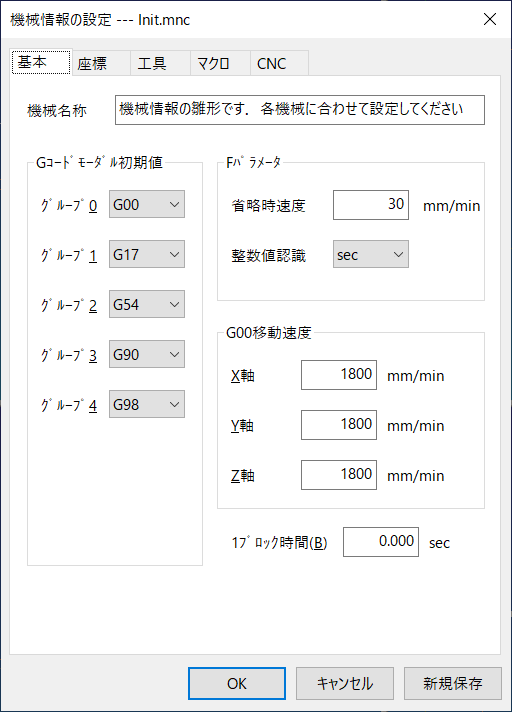
\includegraphics[scale=0.7]{No2/fig/kikai.png}
\caption{機械情報の設定}
\label{fig:kikai.png}
\end{figure}
\end{minipage}

\vspace*{2zh}
 この設定も工作機械ごとに用意しましょう.
現在選択されている機械情報ファイルはツールバーに表示されます(図\ref{fig:select.png}).
加工時間は機械情報ファイルを切り換えるたびに再計算されます.

\begin{figure}[H]
\centering
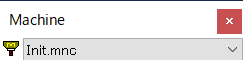
\includegraphics{No2/fig/select.png}
\caption{機械情報ツールバー}
\label{fig:select.png}
\end{figure}

\subsubsection{トレース}

 図\ref{fig:trace.png} はトレースのツールバーです.
とりあえずトレース速度を中速(右から2番目)にしてトレース実行(一番左)を押してみましょう.
どういう手順で加工されていくかを見ることができます.
トレースのスピード調整はリファレンスの表示属性を参照してください.
その他の操作については解説するまでもなく使えると思います.

\begin{figure}[H]
\centering
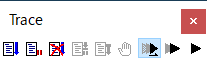
\includegraphics{No2/fig/trace.png}
\caption{トレースツールバー}
\label{fig:trace.png}
\end{figure}

\subsection{穴加工}

 基本編の最後として,固定サイクルでの穴加工データの生成を解説します.
作図レイヤは【\ref{sec:ReadCAD} CADデータの読み込み】と同じで,切削レイヤに穴加工情報を作図します.

 図\ref{fig:sample2.pdf} は矩形の四隅と中央に穴加工を行うための作図データです.
穴加工を行いたい場所を中心に,四隅には半径3mmの円,中央には半径5mmの円を作図しています.
今回はXY原点を示す原点レイヤは作図していません.

 工作機械のXY原点がワークの中央に位置し,CADデータ上でも最大占有領域の中央が原点で良い場合,NCVCがXY原点を補間する機能があります.

\begin{figure}[H]
\centering
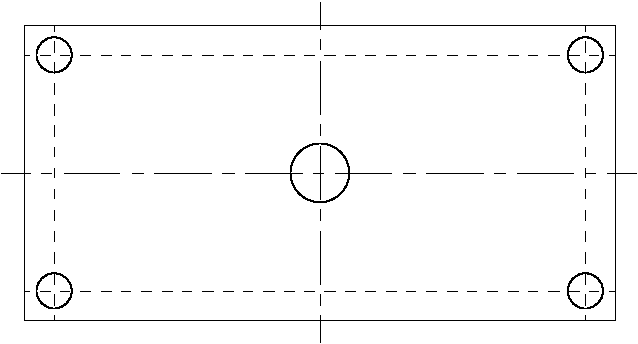
\includegraphics{No2/fig/sample2.pdf}
\caption{穴加工サンプル図形}
\label{fig:sample2.pdf}
\end{figure}

 図\ref{fig:ReadSetup.png}(p.\pageref{fig:ReadSetup.png})の読み込みレイヤ設定と違うのは,[原点データがないとき]の選択肢.
これをエラー以外に設定しておけば,NCVCがXY原点を補間します(図\ref{fig:ReadSetup2.png}).

 ただし,補間はCADデータの最大占有領域から算出されますので,意図しない位置に原点が補間される場合があります.
特別な場合を除き【\ref{DesignCAD} CADでの作図】の通り原点情報を作図することを推奨します.

 穴加工に関する加工条件は【\ref{sec:init.nci} 加工条件の設定】で解説した条件ファイルの[穴加工]タブにて行います(図\ref{fig:hole.png}).
主軸回転数や切削送りなど,穴加工独自に指定可能です.
ここで注目すべき所は[拡張設定グループ]の各種項目.
[円データも穴加工データと見なす]にチェックを入れ,対象となる半径を入力することで,その中心座標に穴加工データを生成します.
従来,穴加工の入力源は点データでしたが,イメージがつかみにくい,点データをDXFに吐けないCADがある等の理由から,
円データでの穴加工が拡張設定となっています.

\vspace*{2zh}
 加工条件が設定できればあとは【\ref{sec:MakeGcode} Gコードの生成】通りです.
図\ref{fig:sample2.png} にシミュレーション結果を示します.
加工条件の[グルーピング順序]を[降順]にすることで半径の大きい中央から固定サイクル命令が生成されています.
また,[大きさごとにコメントを埋め込む]にチェックを入ることで,それぞれの半径ごとにNCVCがコメントを埋め込みますので,
手作業での修正,例えば工具交換命令を埋め込む等,編集の目安となります.

\begin{minipage}{0.5\textwidth}
\begin{figure}[H]
\centering
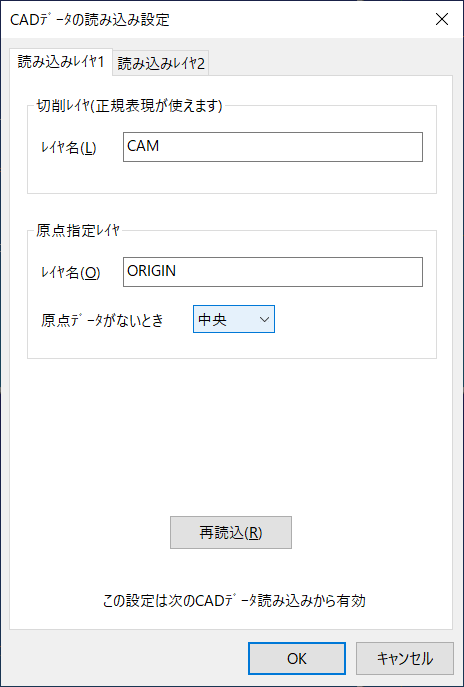
\includegraphics[scale=0.7]{No2/fig/ReadSetup2.png}
\caption{読み込みレイヤ設定2}
\label{fig:ReadSetup2.png}
\end{figure}
\end{minipage}
\begin{minipage}{0.5\textwidth}
\begin{figure}[H]
\centering
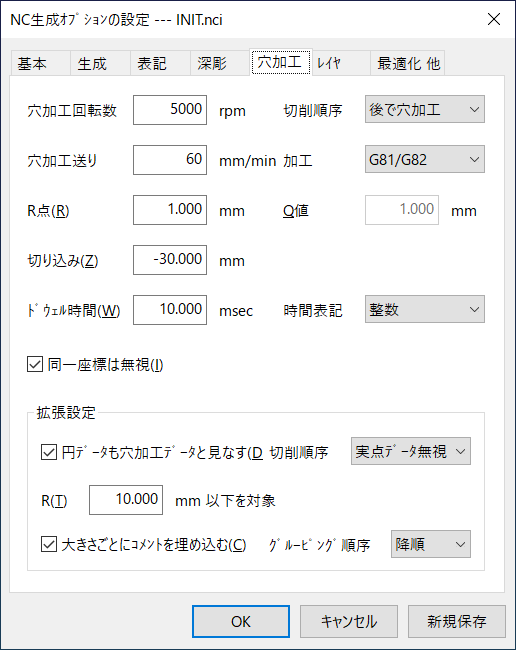
\includegraphics[scale=0.7]{No2/fig/hole.png}
\caption{穴加工の加工条件設定}
\label{fig:hole.png}
\end{figure}
\end{minipage}

\begin{figure}[H]
\centering
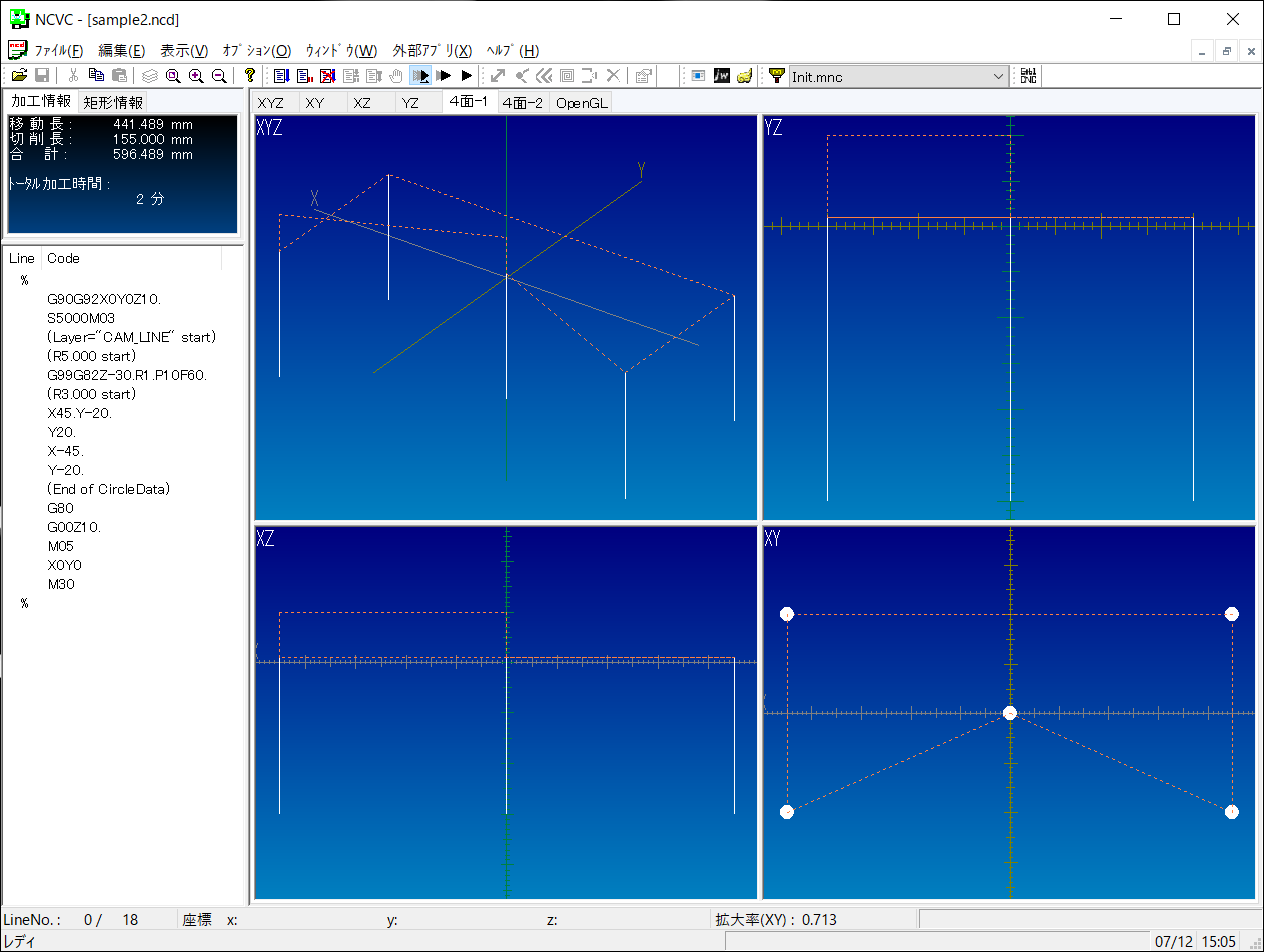
\includegraphics[scale=0.55]{No2/fig/sample02.png}
\caption{穴加工のシミュレーション画面}
\label{fig:sample2.png}
\end{figure}

\newpage

\setcounter{section}{0}
\setcounter{equation}{0}
\setcounter{table}{0}
\setcounter{figure}{0}

%!TEX root = ../NCVC.tex

\mysection{中級編}

\subsection{移動レイヤ}
\label{sec:move}
 NCVCには,原点レイヤ・切削レイヤの他にあと3つのレイヤ情報を読み込む機能があります.
ここではそのうちの2つ,加工開始位置指示レイヤと強制移動指示レイヤを解説します.

\subsubsection{加工開始位置指示レイヤ}
 図\ref{fig:sample3.pdf} のような加工を考えます.
原点はワーク矩形左下で円を内側から螺旋状に切削したいのですが,これだけでは思ったようなGコードを生成できません.

 NCVCは次の切削データを検索するとき,現在位置に最も近い座標を検索します.
したがって,原点から一番近い座標である外側の座標からGコードの生成を始めます.

 これを回避するため,NCVCでは[加工開始位置指示レイヤ]を用意しています.
CADでの作図で原点・切削の両レイヤとは別のレイヤを用意し,円を1つ作図して下さい.
レイヤ名も設定です.作図方法は原点指示と同じ,円の中心が加工開始座標となります.

 NCVCでの設定は【\ref{sec:ReadCAD} CADデータの読み込み】と同じです.
[読み込みレイヤ2]のタブをクリックし,NCVCが読み込むレイヤ名を設定して下さい(図\ref{fig:ReadSetup3.png}).
[読み込みレイヤ2]の設定は必須ではありませんが,CAD側で意図的に作図しない限りNCVCは読み込みませんので,常にこの設定にしても問題ありません.
レイヤ名は,原点・切削の両レイヤと同様に任意です.CAD側の設定と合わせて下さい.
加工開始指示を指示したシミュレーション結果を図\ref{fig:sample3.png} に示します.

\begin{minipage}{0.5\textwidth}
\begin{figure}[H]
\centering
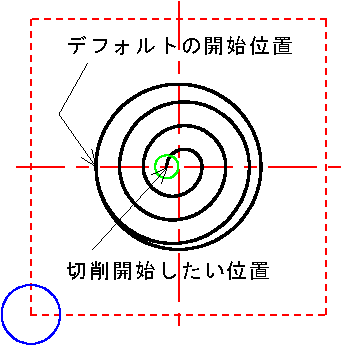
\includegraphics{No3/fig/start-crop.pdf}
\caption{サンプル図形}
\label{fig:sample3.pdf}
\end{figure}
\end{minipage}
\begin{minipage}{0.5\textwidth}
\begin{figure}[H]
\centering
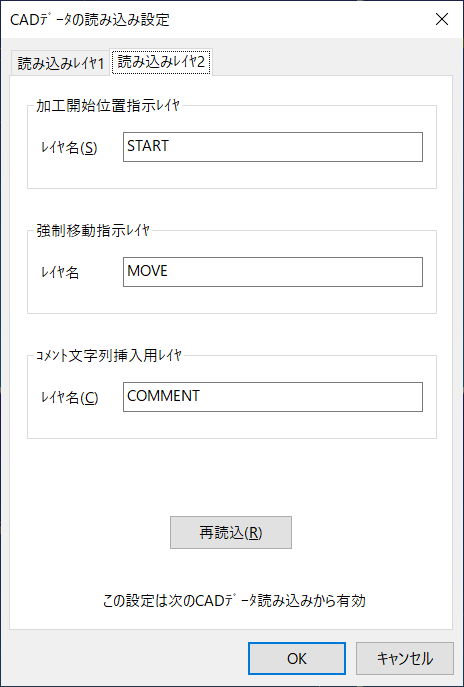
\includegraphics[scale=0.7]{No3/fig/ReadSetup3.png}
\caption{読み込みレイヤ設定}
\label{fig:ReadSetup3.png}
\end{figure}
\end{minipage}

\begin{figure}[H]
\centering
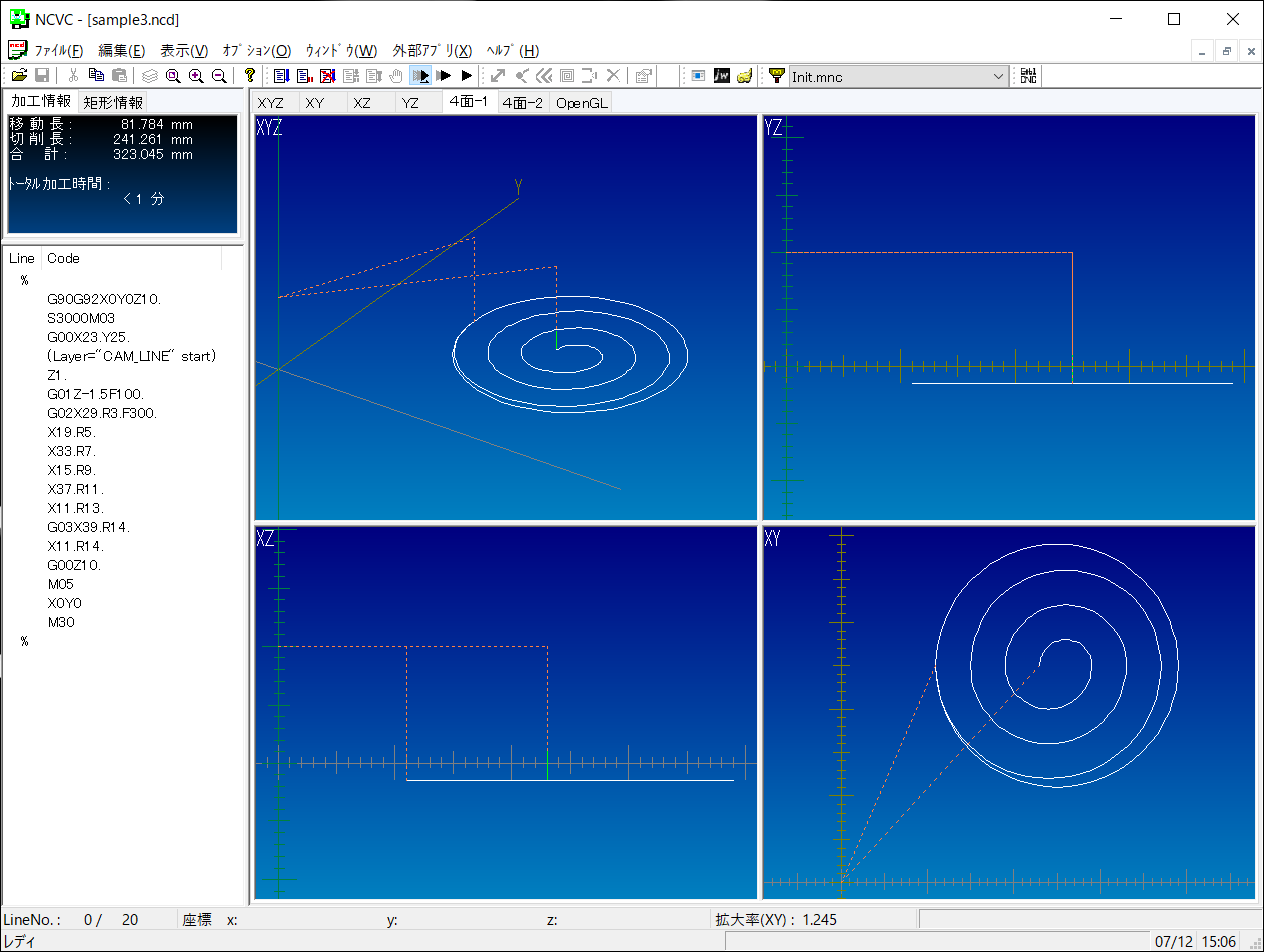
\includegraphics[scale=0.55]{No3/fig/sample3.png}
\caption{加工開始位置を追加したGコードシミュレーション画面}
\label{fig:sample3.png}
\end{figure}

 加工開始位置指示レイヤにはもう1つ機能があります.
例えば図\ref{fig:approach-img.png} のようなワーク形状の場合,原点からの最短移動ではワークに干渉してしまいます.
この場合,図\ref{fig:approach.pdf} のように干渉しないような移動軌跡を加工開始位置指示レイヤに作図することで,原点からの移動動作を制御することができます.
Z軸の初期座標を上げることで回避できる場合もあります.用途に応じてご使用下さい.

\begin{minipage}{0.5\textwidth}
\begin{figure}[H]
\centering
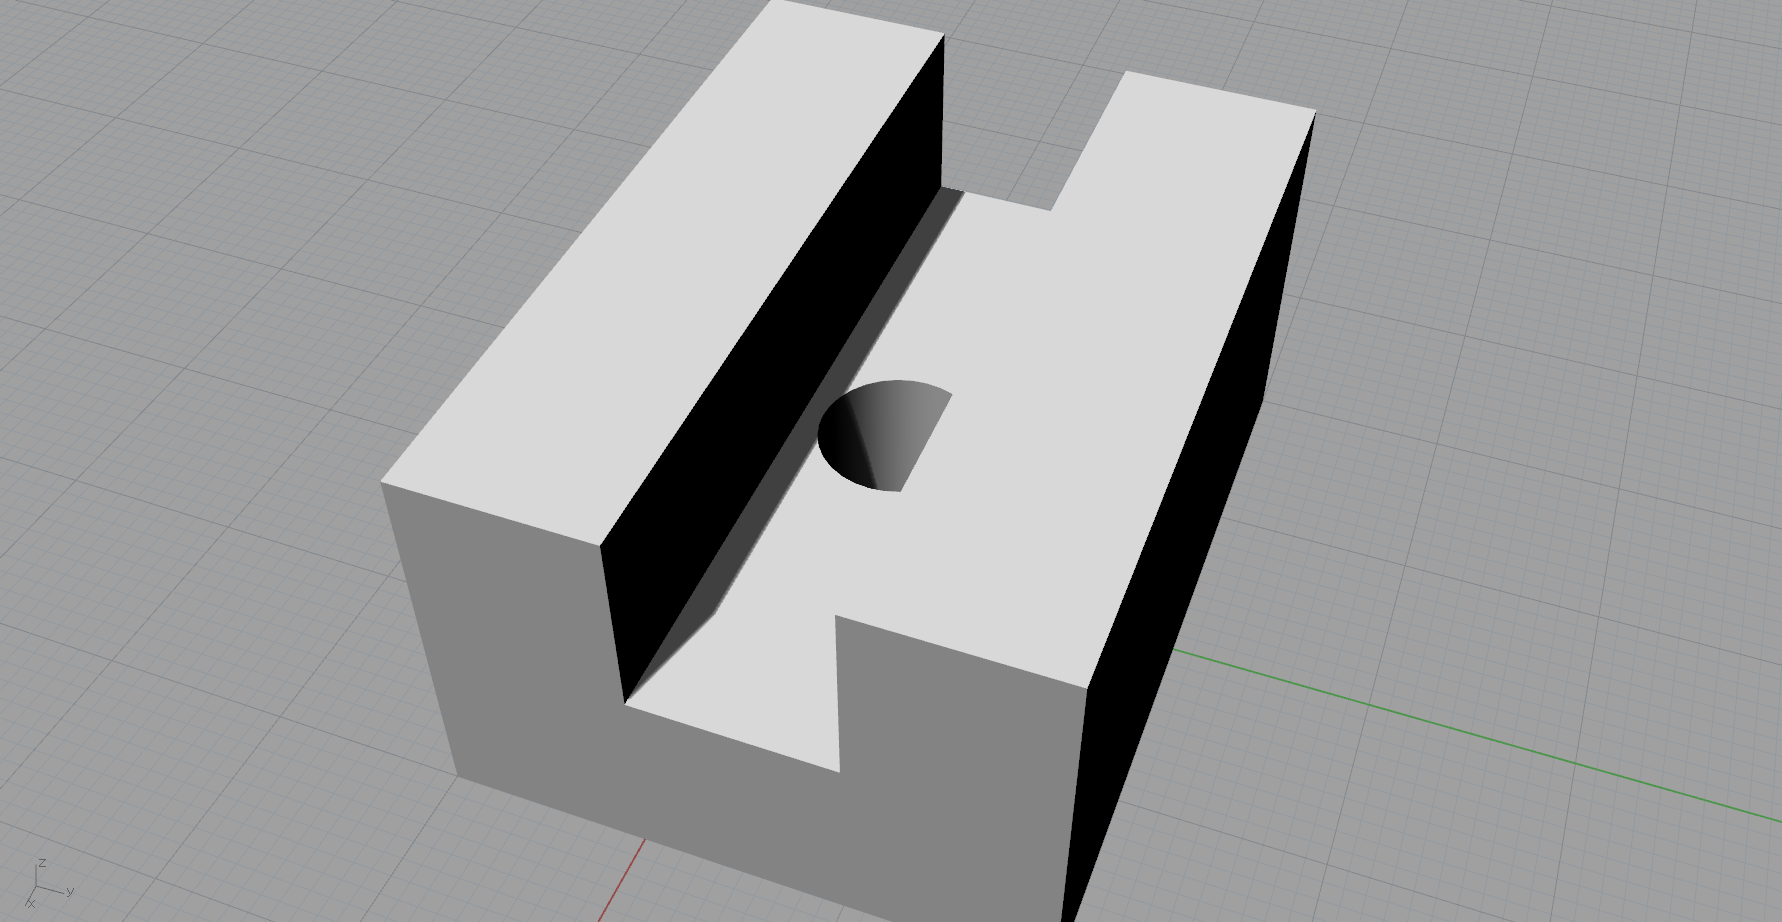
\includegraphics[width=\textwidth]{No3/fig/approach-img.png}
\caption{サンプルイメージ図}
\label{fig:approach-img.png}
\end{figure}
\end{minipage}
\begin{minipage}{0.5\textwidth}
\begin{figure}[H]
\centering
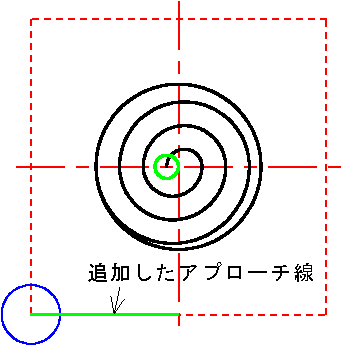
\includegraphics{No3/fig/approach-crop.pdf}
\caption{アプローチ線}
\label{fig:approach.pdf}
\end{figure}
\end{minipage}

\begin{figure}[H]
\centering
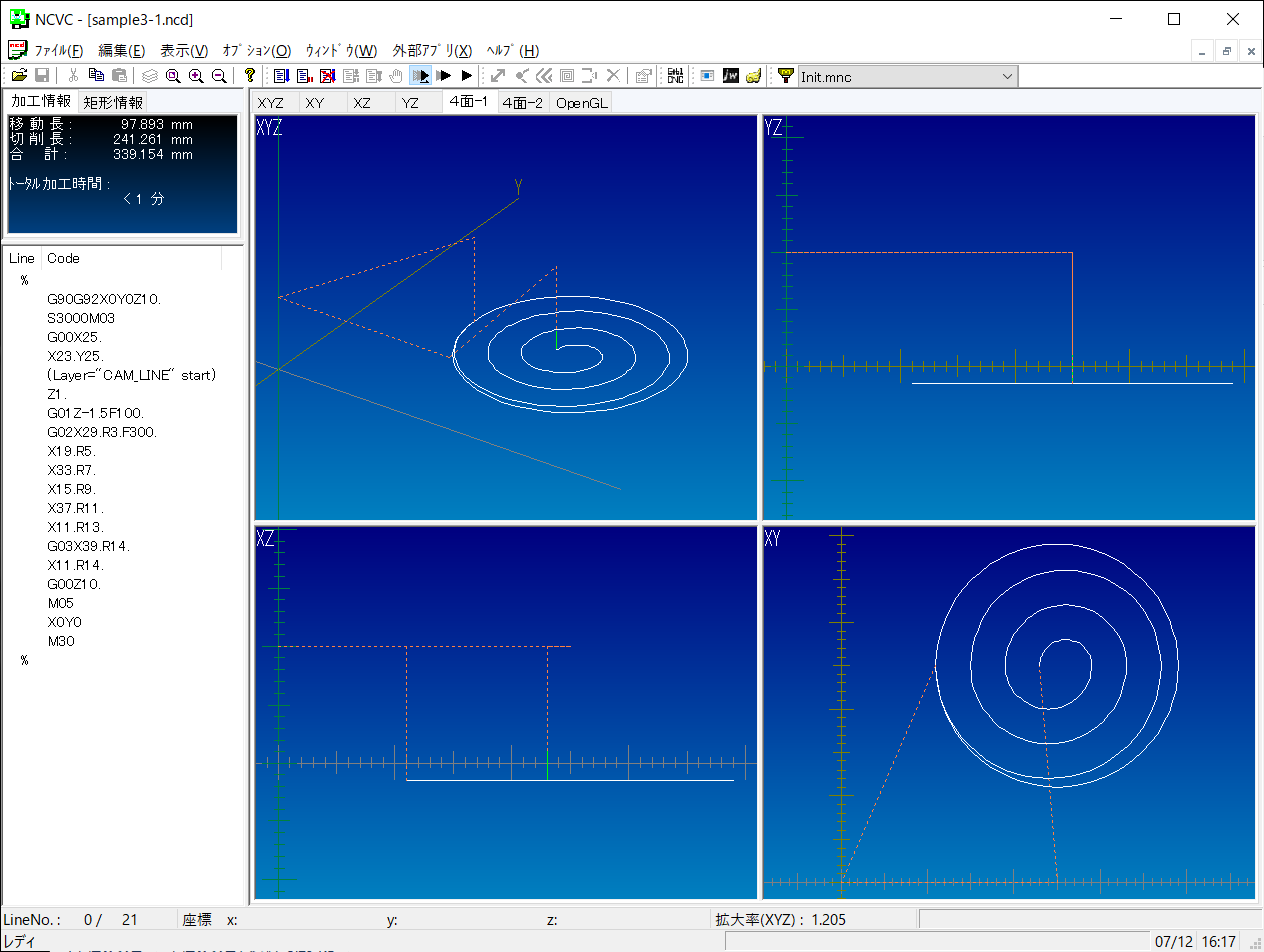
\includegraphics[scale=0.55]{No3/fig/sample3-1.png}
\caption{アプローチ線を追加したGコードシミュレーション画面}
\label{fig:sample3-1.png}
\end{figure}

\subsubsection{強制移動指示レイヤ}
 図\ref{fig:sample3-1.png} のシミュレーション結果を見ても解る通り,原点へ戻るときもワークと干渉してしまう可能性があります.
加工開始位置指示レイヤは,最初の加工位置やアプローチを指示するものでしたが,
強制移動指示レイヤは,次の切削データの検索途中でNCVCに移動を指示する情報となります.
つまり,次の切削領域への移動,Z軸の上下が必要なときに強制移動指示レイヤが参照されます.

\begin{minipage}[t]{0.5\textwidth}
 強制移動指示レイヤは線データのみを認識します.
図\ref{fig:ReadSetup3.png} で設定した移動レイヤに作図して下さい.
また,必ず切削データと接続されていなければなりません.
図\ref{fig:move.pdf} は切削が終わったあとの移動軌跡を作図したものです.
\end{minipage}
\begin{minipage}[t]{0.5\textwidth}
\vspace*{-2zh}
\begin{figure}[H]
\centering
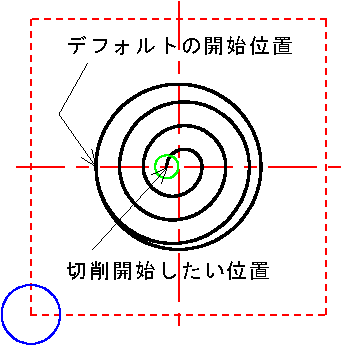
\includegraphics{No3/fig/move-crop.pdf}
\caption{強制移動指示レイヤを追加}
\label{fig:move.pdf}
\end{figure}
\end{minipage}

\begin{figure}[H]
\centering
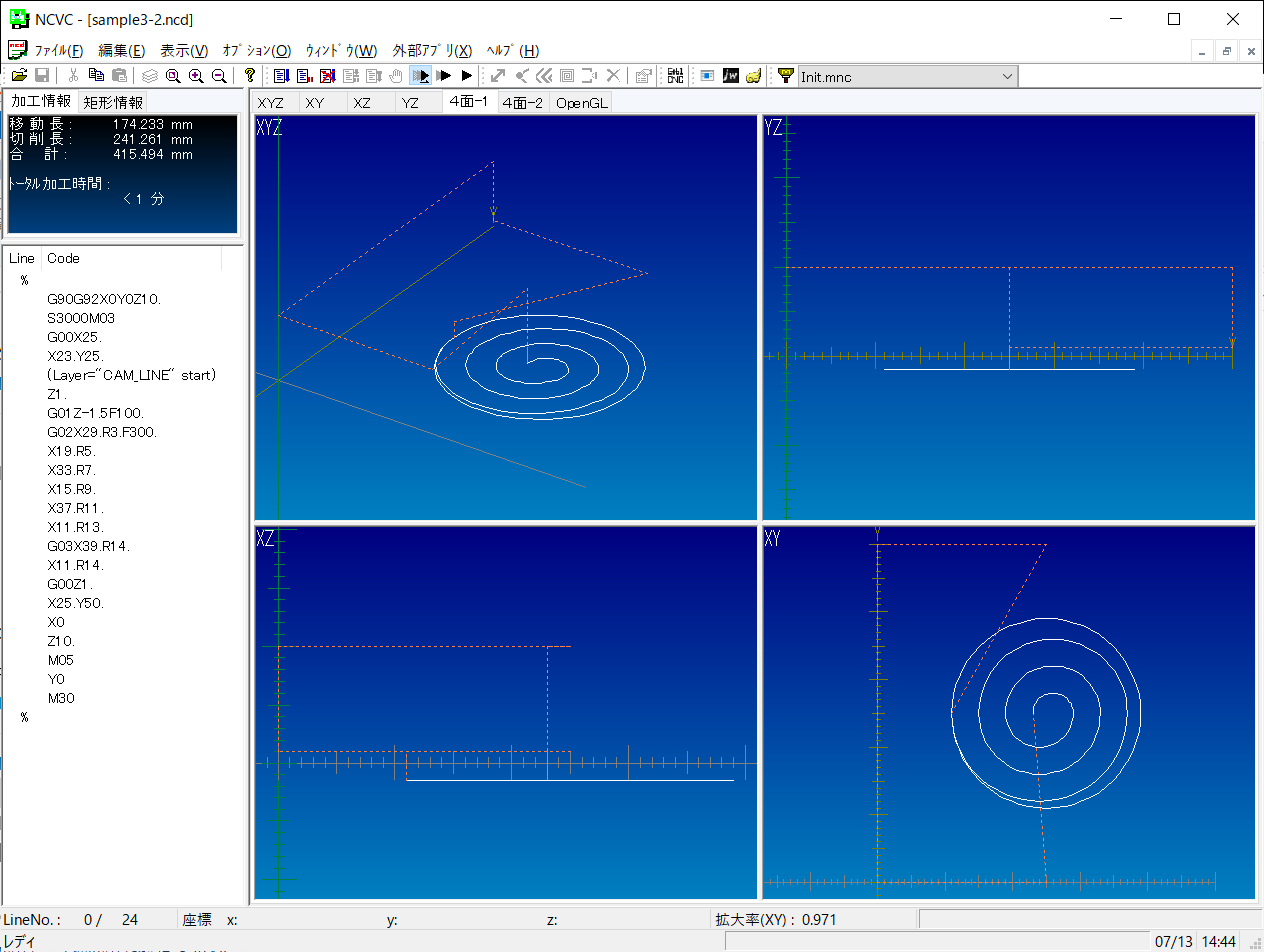
\includegraphics[scale=0.55]{No3/fig/sample3-2.png}
\caption{強制移動データを追加したGコードシミュレーション画面}
\label{fig:sample3-2.png}
\end{figure}

\begin{minipage}[t]{0.5\textwidth}
 図\ref{fig:sample3-2.png} のシミュレーション結果から,強制移動指示レイヤがR点で移動していることが解ります.
この設定は加工条件の[レイヤ]タブにあります.
今回の例では[イニシャル点復帰]が正解ですが,強制移動指示レイヤは大抵の場合,次の切削領域への移動制御に使われるため,
通常は[R点復帰]で問題無いと思います.
\end{minipage}
\begin{minipage}[t]{0.5\textwidth}
\vspace*{-2zh}
\begin{figure}[H]
\centering
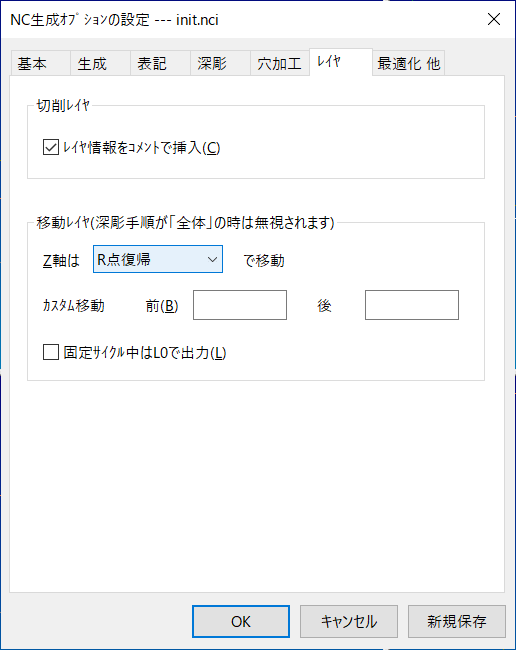
\includegraphics[scale=0.7]{No3/fig/move-setup.png}
\caption{強制移動指示レイヤのZ値設定}
\label{fig:move-setup.png}
\end{figure}
\end{minipage}

\begin{itembox}[l]{ここまでの【まとめ】}
(1) 加工開始位置指示レイヤ
\begin{itemize}
\item 加工開始位置を円で示す,またはアプローチ線を作図
\item 円や線は切削データと繋がって無くても良い
\end{itemize}
(2) 強制移動指示レイヤ
\begin{itemize}
\item 切削データが途切れ,次の切削領域へ移動するとき,参照される
\item 切削データと繋がっていなければならない
\item 強制移動指示レイヤのZ値は加工条件の設定による
\end{itemize}
\end{itembox}

\subsection{Gコード(文字)の埋め込み}
 NCVCで生成されるGコードは,基本的に位置決めと直線・円弧補間のG00~G03,固定サイクルG81~の一部だけです.
ここでは工作機械の特殊コード(例えばATCによるツール交換コード)やカスタムマクロ呼び出しコードなど,
生成されるGコードに任意の文字列を埋め込む方法を解説します.

\begin{minipage}[t]{0.5\textwidth}
 作図方法は至極簡単.図\ref{fig:moji.pdf} に示すように,埋め込みたいオブジェクト(線や円弧)の端点に文字を作図するだけです.
文字データは原点レイヤ以外,すなわち,切削レイヤと2つの移動レイヤ,
それから【\ref{sec:move} 移動レイヤ】の節で解説した最後のレイヤである[コメント文字列挿入用レイヤ](p.\pageref{fig:ReadSetup3.png} 図\ref{fig:ReadSetup3.png})に作図することができます.

 埋め込みタイミングは,文字専用レイヤである[コメント文字列挿入用レイヤ]が先に参照され,次に各レイヤタイプに属する文字データが参照されます.
[コメント文字列挿入用レイヤ]に書かれた文字はその名の通りGコードに対するコメントと見なされ,カッコで括られます.その他のレイヤに書かれた文字はそのまま出力されます.
なお,文字データは1行で作図する必要がありますが,複数行の任意Gコードを埋め込みたい場合は改行位置で ``\,\textbackslash n\,'' と入力して下さい.
\end{minipage}
\begin{minipage}[t]{0.5\textwidth}
\vspace*{-1zh}
\begin{figure}[H]
\centering
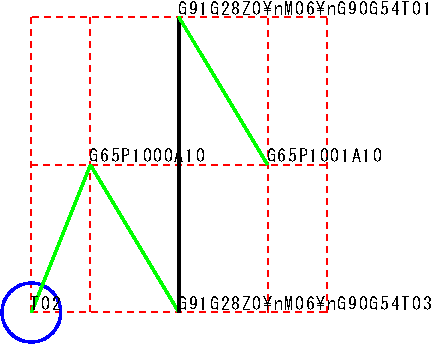
\includegraphics{No3/fig/moji-crop.pdf}
\caption{文字埋め込みサンプル}
\label{fig:moji.pdf}
\end{figure}
\end{minipage}

 図\ref{fig:moji.pdf} の作図から生成されるGコードは以下の通りです.
反転部分が文字情報から拾われたデータです.
作図は簡単ですが,文字を埋め込むレイヤと場所(タイミング)には若干知恵を絞る必要があります.

%\begin{multicols}{2}
%\begin{screen}
\begin{minipage}[t]{0.5\textwidth}
\begin{lstlisting}[numbers=none,label=lst:moji.txt]
%
G90G54G92X0Y0Z10.
M8
M68
S3000M3
T02
G00X10.Y25.
G65P1000A10
X25.Y0
G91G28Z0
M06
G90G54T03
Z1.
G01Z-2.F100
 右へ続く
\end{lstlisting}
%\columnbreak
\end{minipage}
\begin{minipage}[t]{0.5\textwidth}
\begin{lstlisting}[numbers=none]
Y50.F300
G91G28Z0
M06
G90G54T01
G00Z1.
X40.Y25.
G65P1001A10
Z10.
M9
M5
X0Y0
M30
%
\end{lstlisting}
\end{minipage}
%\end{screen}
%\end{multicols}

\begin{figure}[H]
\centering
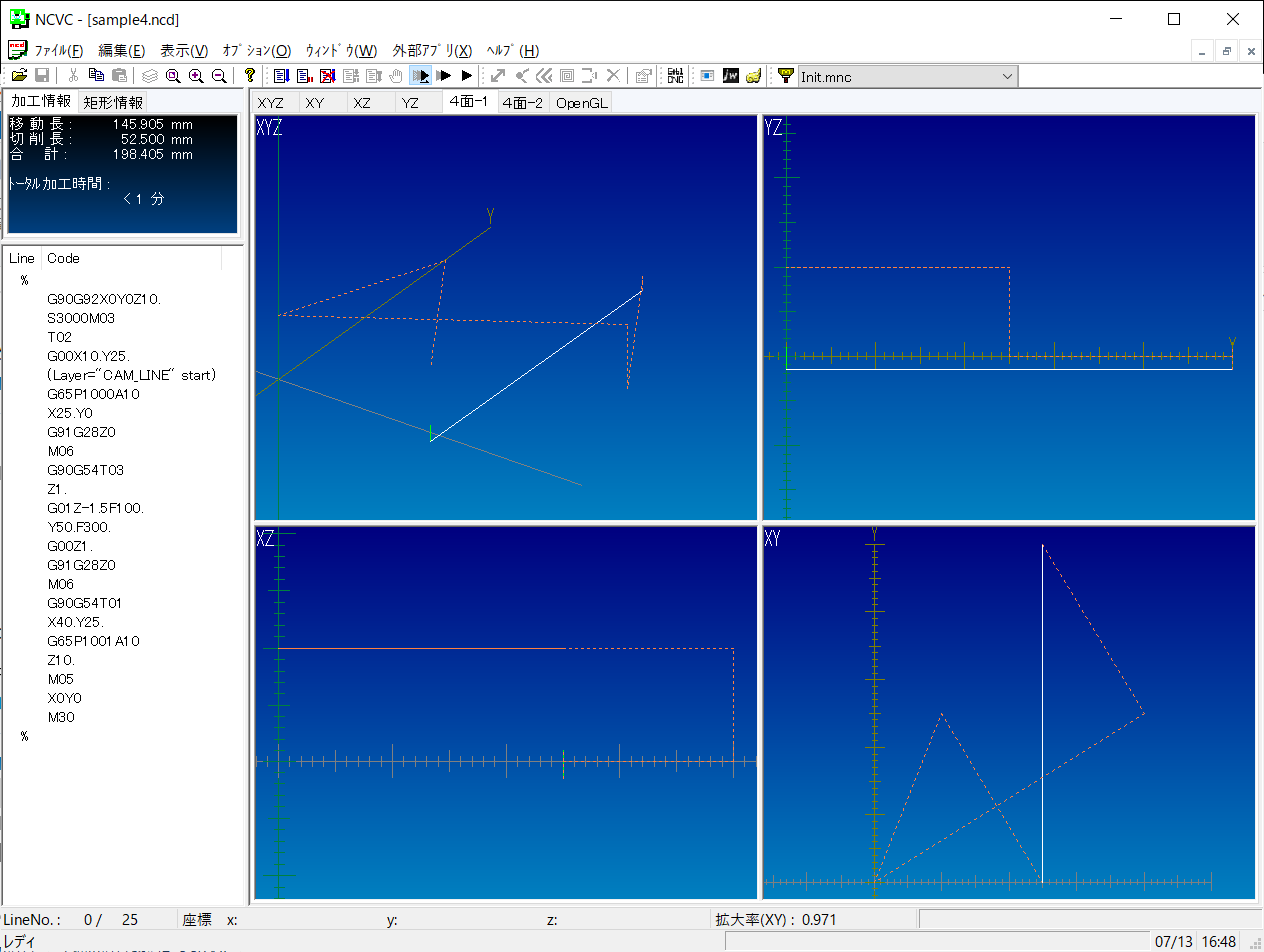
\includegraphics[scale=0.55]{No3/fig/sample4.png}
\caption{Gコードシミュレーション画面}
\label{fig:sample4.png}
\end{figure}

\subsection{深彫切削(Z軸ステップ切削)}
\newpage

\setcounter{section}{0}
\setcounter{equation}{0}
\setcounter{table}{0}
\setcounter{figure}{0}

%!TEX root = ../NCVC.tex

\mysection{応用編}

\subsection{方向制御}
 結論から言うと,普通の方法では方向制御できません.
例えば1つの座標に複数のオブジェクトが接続されている場合,NCVCが最初にどれを選択するかは内部で独自に決定されます.
ここでは応用編の第一弾としてムリヤリ(?)方向制御を行う方法を解説します.

\begin{minipage}[t]{0.5\textwidth}
 図\ref{fig:direction}を見てください.
中心の加工原点と左下の加工開始を示す円データ,五角形の線データがあります(それ以外は補助線).
一見して普通の作図,\ref{sec:move}節で解説した移動レイヤだけに見えますが,実は複数レイヤ処理との合わせ技で作図されています.
図\ref{fig:direction.png} は図\ref{fig:direction}のCADデータを読み込み,レイヤ表示で切削レイヤの2つ目を非表示にした状態を表しています.
\end{minipage}
\begin{minipage}[t]{0.5\textwidth}
\vspace*{-2zh}
\begin{figure}[H]
\centering
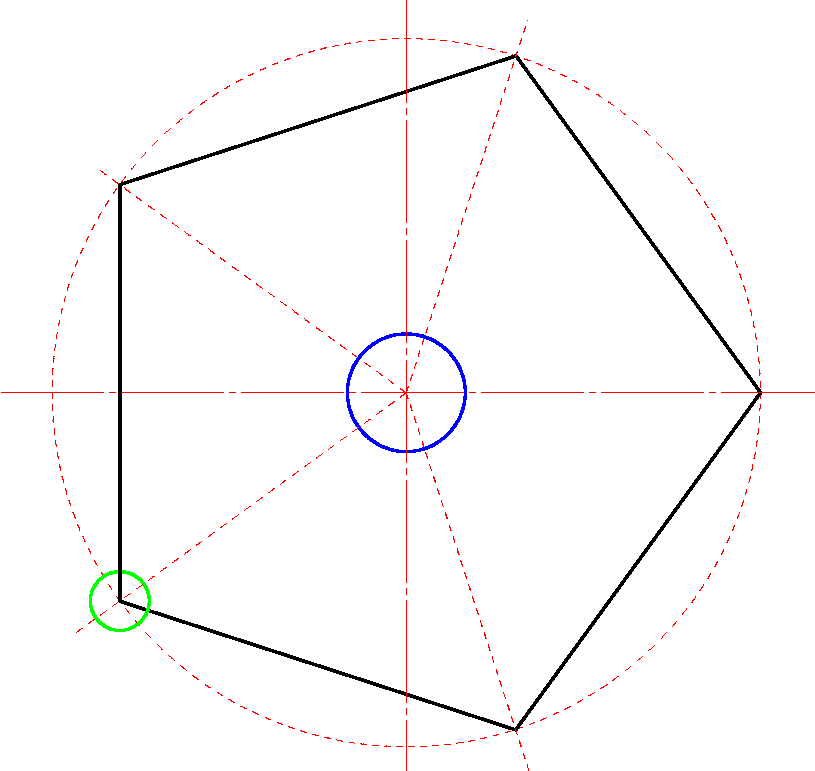
\includegraphics[width=\textwidth]{No4/fig/direction-crop.pdf}
\caption{方向制御作図例}
\label{fig:direction}
\end{figure}
\end{minipage}

\begin{figure}[H]
\centering
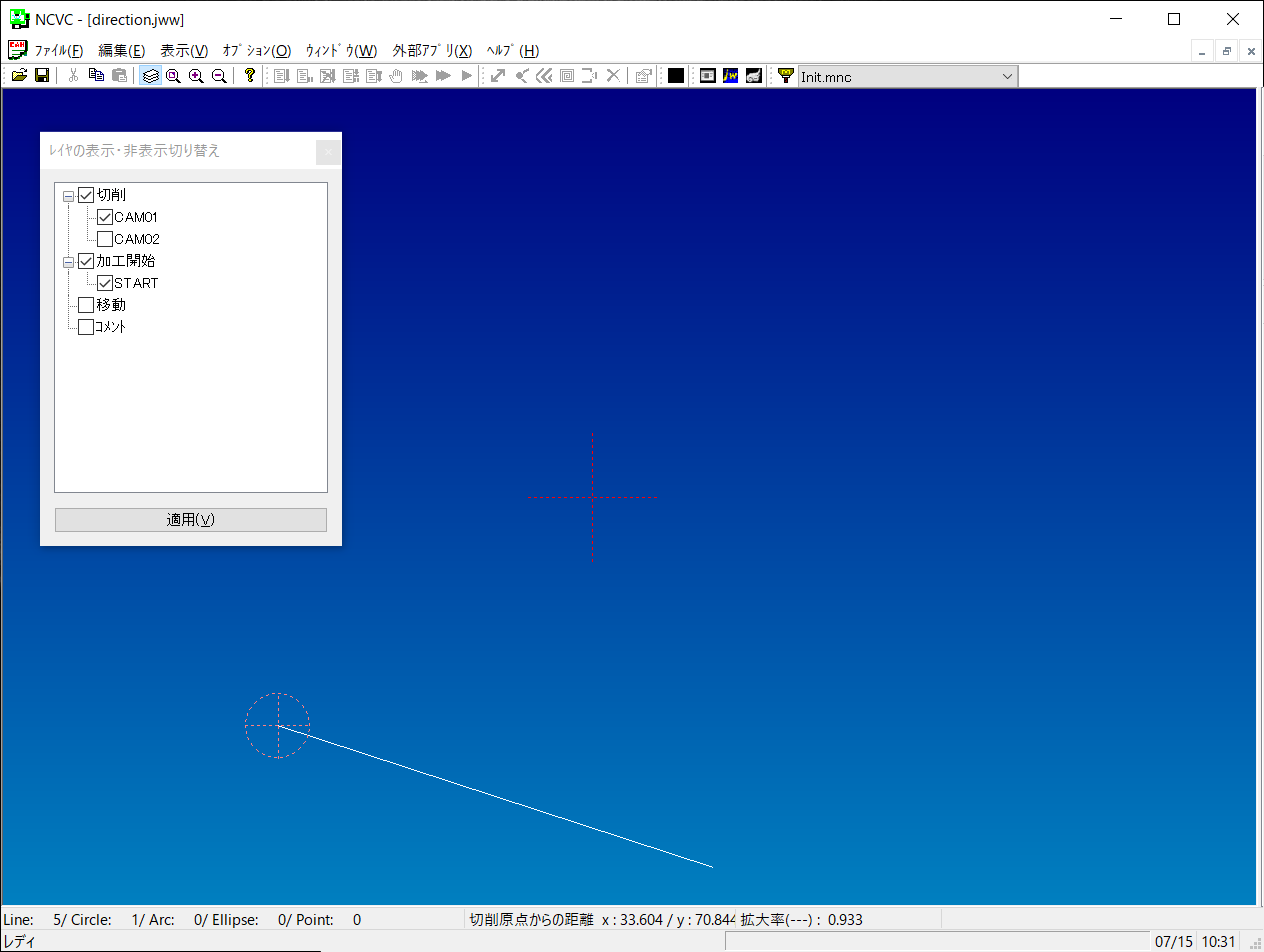
\includegraphics[scale=0.55]{No4/fig/direction.png}
\caption{複数レイヤを読み込んだ状態}
\label{fig:direction.png}
\end{figure}

\begin{minipage}[t]{0.5\textwidth}
 もうお解りですね.開始したい座標に複数のオブジェクトがあれば,それを違うレイヤに作図し,方向が明確に示せるようにすればOKです.
ただし,複数レイヤ処理を行う必要があるので,単一条件でのNC生成では希望通り生成できません.
【\ref{sec:multi-layer} 複数レイヤ処理】で解説した拡張NC生成,[レイヤごとのZ座標指定]か[レイヤごとの切削条件]で処理する必要があります.
どちらの場合でも同じZ値,または,同じ条件を割り当てることができます(図\ref{fig:direction-setup}).
\end{minipage}
\begin{minipage}[t]{0.5\textwidth}
\vspace*{-2zh}
\begin{figure}[H]
\centering
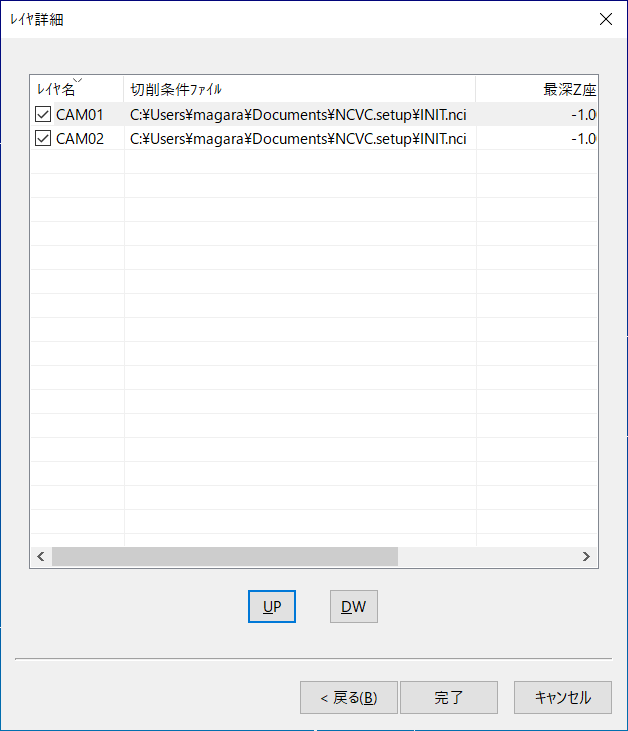
\includegraphics[scale=0.6]{No4/fig/direction-setup.png}
\caption{2つの切削レイヤに同じ加工条件を割り当て}
\label{fig:direction-setup}
\end{figure}
\end{minipage}

\vspace*{2zh}
\begin{minipage}[t]{0.6\textwidth}
 もう1つ,裏技的というより,これぞムリヤリですが(自爆)要するに1つの座標に2つ以上のオブジェクトを作図しなければ良いだけで,
例えば図\ref{fig:direction2} のように矩形切削の方向を指示したい場合,影響の無い範囲内で他方の座標をずらしてやれば良いのです.
前の切削領域からの最短距離ならNCVCが自動で検索します.明確に指示したい場合は【\ref{sec:move} 移動レイヤ】が使えます.
\end{minipage}
\begin{minipage}[t]{0.4\textwidth}
\vspace*{-2zh}
\begin{figure}[H]
\centering
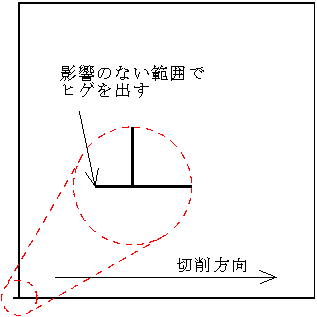
\includegraphics[width=\textwidth]{No4/fig/direction2-crop.pdf}
\caption{矩形切削例}
\label{fig:direction2}
\end{figure}
\end{minipage}

\vspace*{2zh}
 どちらにしてもあまり格好の良い方法ではありませんね...

\subsection{形状切削}
 方向制御と同じく形状切削についてもNCVCでは生成できません.
一般的にCADでは完成された形状を作図しますが,実際の加工では工具の半径を考慮しなければなりません.
特に島加工・ポケット加工については,CADで作図した形状情報からNCVCが加工データを生成できません.
NCVCはCADのデータを工具の軌跡データと扱うのです.

 もうカンの良い皆様ならお気づきだと思います.
NCVCで形状切削の加工データを得るには,今度こそCADの力を存分に借りる必要があります.
図\ref{fig:keijyou.pdf} は【\ref{sec:hole} 穴加工】のサンプルデータ(p.\pageref{fig:sample2.pdf})からポケット加工のデータを得るための作図例です.
工具半径や必要な肉厚を考慮しつつCADの複線機能を駆使して作図しました.
面倒そうですが慣れると意外と簡単に作図できます\footnote{ご使用のCADの性能や習熟度次第ですが...}.
削りすぎにはくれぐれもご注意を(体験談).
削り残しも作図段階でチェックできませんが
\footnote{Jw\_cad の場合,円の作図で半径を入力すれば,これから作図しようとする円が表示されます.
これを工具に見立ててマウスを動かせば簡易チェッカ(?).無論補助レイヤにて工具円を書きまくるのが確実デス.},
NCVCのシミュレーション画面もワイヤー表示なので,どのみちチェックできませんね(自爆x2)

\begin{figure}[H]
\centering
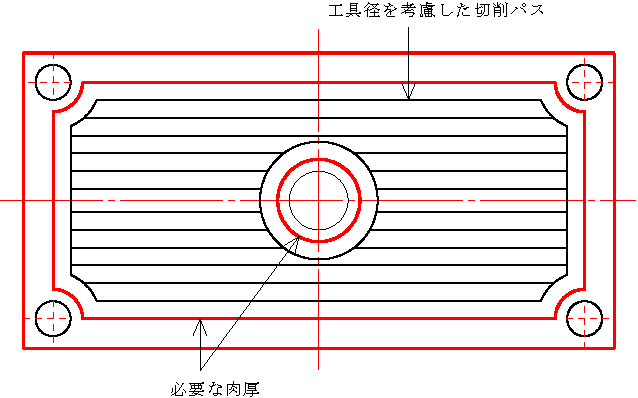
\includegraphics{No4/fig/keijyou-crop.pdf}
\caption{ポケット加工作図例}
\label{fig:keijyou.pdf}
\end{figure}

\vspace*{2zh}
\begin{itembox}[l]{ここまでの【まとめ】}
\begin{itemize}
\item 方向制御と形状切削は,CADの作図次第
\item スマートに指示するにはもう少しNCVCの進化を待つ必要がある
\end{itemize}
\end{itembox}

\newpage

\setcounter{section}{0}
\setcounter{equation}{0}
\setcounter{table}{0}
\setcounter{figure}{0}

%!TEX root = ../NCVC.tex

\mysection{パワーユーザ編}

\subsection{スクリプト作成のすすめ}

\subsubsection{まえがき}
 awk(オーク), Perl(パール), Ruby(ルビー)これらの名前を聞いたことがあるでしょうか?
この3つを知らなくても,BasicやC/C++なら聞いたことがあるかと思います.
これら全てプログラミング言語で,先に挙げた3つの言語は特にテキストファイルの処理に優れた能力を発揮し,しかもそれらの処理を簡単に記述できるという特徴を持ったプログラミング言語です.

 さて,「プログラミング言語」と聞いて尻込みしているアナタ!
それは大きな誤解と難しいという先入観だと思います.
冒頭でも述べた通り,テキストファイルの処理に優れた能力を発揮できる非常に良く考えられた言語で,
目的にもよりますが極端な話し,たった1行でも十分実用可能なプログラムを作成することができます.
\ref{sec:multi-layer}節で少しだけ登場した正規表現がサポートされているので強力な文字列のパターンマッチングが可能,
つまり,テキストファイルの中から必要な情報を検索したり置換するといったことが簡単に記述できます.

 これがNCVCの解説書とどう関係があるのか?
答えは簡単,NCVCが吐くGコードがショボイから(自爆)...たしかにそれもありますが(汗),
例えば特殊なコード変換や埋め込み,サポートされていない機能の補間など,小粒だがピリリと気の利いた自分専用のツールを作ってみよう!
というのがこの章の目的です.
そう,Gコード(NCファイル)はテキストファイルです.
プログラミング可能な一定のルールがあるなら,もうメモ帳でシコシコ手修正する必要はありません.
\\ \\
 本解説書では,BasicやC/C++のプログラミング言語と区別するため,以後,スクリプト言語と称します.

\subsubsection{例題}
 とエラそうなことを書きましたが,ここで言語仕様等を書いてはキリが無いので,言語自体の解説は専門書にオマカセします.
また,スクリプト言語といえばPerlが有名ですが,著者はawkヲタク.
例題もただの検索や置換だけならメモ帳でもできるので,ちょっと複雑な例題を用意しました.
おかげで前述の「たった1行でも」というフレーズは実現できませんでした(ゴメンナサイ).

 では早速例題のテーマですが,『シーケンス番号の追加』とします.
NCVCにもシーケンス番号を付加する生成オプションがありますが,コメント行などお構いなしに付加するため,この例題では次に示す行にシーケンス番号を付加しない仕様とします.

\begin{itemize}
\item O番号(プログラム番号),``\,\%\,'',カッコ``\,(\,''で始まる行
\item 空行
\end{itemize}

 awkスクリプトで書くと以下のようなリストになります.
これをメモ帳などで入力し,ファイルとして保存しておきましょう.
一見して解る通り,BasicやC/C++では必要なファイルのオープンや1行ずつ読み込んでループ等の処理は必要ありません.
awkで必要なのは条件パターンとその条件に対する処理(アクション)だけです.

\newpage
\begin{lstlisting}[caption=num.awk,numbers=none,label=lst:num.awk]
BEGIN {         # 最初に実行されるブロック
  num=1000;       # シーケンス番号の初期値
  add=5;          # 増分値
}
/^O|^\(|^%/ || length($0)==0 {  # シーケンス番号を付加しない条件
  print $0                    # 1行そのまま出力($0は入力1行全てを表す)
  next                        # 次の処理(入力)へ
}
{                               # 条件パターン無しブロック(上記条件以外)
  printf("N%04d", num);       # N に続く4桁の数字を出力(改行無し)
  print $0;                   # 1行そのまま出力
  num += add;                 # 増分の加算
}
\end{lstlisting}

\subsubsection{実行環境}
 もともとこれらスクリプト言語はUNIX文化で培われたものです.
UNIXにはほぼ標準で用意されていますが,Windowsで実行するには,それぞれの処理系をインストールする必要があります.
awkならGNUawk(gawk)が有名ですのでインストールしておいて下さい
\footnote{大規模なシステムではないので,展開して実行ファイル(EXE)をパスの通ったフォルダに移動させる,もしくはスクリプトと同じ場所に置くだけで良い}.

 実行環境が整えば,Windowsスタートメニューからコマンドプロンプト
\footnote{Windowsのバージョンによって違います.DOS窓のこと}
を開き,以下のように入力します.

\vspace*{1zh}
\begin{shadebox}
gawk -f \textit{ScriptName}.awk \textless \textit{Input-file}
\end{shadebox}

\vspace*{1zh}
 希望通りに変換されたGコードが表示されましたか?
必要なら

\vspace*{1zh}
\begin{shadebox}
gawk -f \textit{ScriptName}.awk \textless \textit{Input-file} \textgreater \textit{Output-file}
\end{shadebox}

\vspace*{1zh}
とすることで,\textit{Output-file} に示すファイルに書き出されます.

\subsubsection{あとがき}
 これくらいの例題だけでは,自分がしたい処理を書くことは正直難しいと思います.
けれども,スクリプト言語はGコードの置換処理だけでなくその他事務処理等にも応用できます.
得られるものは大きいのでぜひチャレンジしてみて下さい.

 新たに挑戦する場合は先人たちの知恵が大いに参考になると思います.
NCVCのWebページにはたくさんのスクリプトが掲載されていますのでご参考に.
また,NCVCからスクリプトが簡単に実行できるラッパーもあります.Scriptoriumのドキュメントも併せてご参考に.

\subsection{アドイン作成のすすめ}
 アドイン作成とはDLLの作成を意味し,NCVC本体の機能を内部的に拡張することができます.
前節のスクリプト言語とは対照的に高度なプログラミング知識が要求されますので,「DLLって何?」という方は表\ref{table:addin} の一覧だけ眺めてあとは読み飛ばしてもかまいません.

 さてアドインの作成ですが,NCVCのWebページからSDKをダウンロードし,インクルードファイルとインポートライブラリを各開発環境にインストールして下さい.
基本的にメニューイベント型のアドイン,つまり,アドイン側の初期化関数内で必要なメニューを登録し,メニューが選択されたときNCVCから登録された関数が呼ばれるという仕組みです.
関数一覧などSDKの詳細は別途SDKマニュアルを参照して下さい.

 【アドイン作成のすすめ】のタイトル通り,アドインによる機能拡張の有効性,特にCADデータのインポートについて述べると,『DXF形式で保存する必要が無くなる』が上げられます.
加工データ生成の初期段階ではCADソフトとの連携が重要ですが,\ref{sec:DesignCAD}節で述べたとおりCADソフト独自形式とDXF形式と併用しての保存は非常に煩わしいと感じるでしょう.
さらに,NCVCには現在開いているファイルがNCVC以外で変更されると,その変更を検知してアナウンスする機能があります.
CADソフト独自形式をインポートできることで,この機能を有効に使うことができます.

 ということで,ご使用CADのデータ形式が解ればぜひアドイン作成にチャレンジしてみましょう.
他,「こういう機能拡張を」というのがあれば腕試しにいかが?

\begin{table}[H]
\caption{アドイン一覧}
\label{table:addin}
\centering
\begin{tabular}{|l|l|l|}
\hline
\multicolumn{1}{|c|}{アドイン名} & \multicolumn{1}{c|}{概要} & \multicolumn{1}{c|}{備考} \\ \hline \hline
SendNCD    & Gコードのシリアル送信 & インストーラ付属 \\ \hline
ReadJW     & Jw\_cadデータ(JWC/JWW)のインポート &  〃 \\ \hline
ReadCSV    & CSV形式の座標データインポート & 次回インストーラ付属 \\ \hline \hline
ReadDWG    & AutoCADデータ(DWG)のインポート & 開発中断(中止) \\ \hline
SolveTSP   & 巡回セールスマン問題の解法を用いた穴加工の移動最適化 & プロト完成後開発一時中断 \\ \hline
ReadGerber & 基板加工データ(ガーバー)のインポート & 構想のみ \\ \hline
\end{tabular}
\end{table}

\newpage

\end{document}
